\documentclass[a4paper, 12pt]{article}

% Pacotes essenciais
\usepackage[utf8]{inputenc}
\usepackage[T1]{fontenc}
\usepackage[portuguese, english]{babel}
\usepackage{graphicx}
\usepackage{url}
\usepackage{xurl}
\usepackage{ragged2e}
\usepackage{amsmath,amssymb,amsfonts}
\usepackage{verbatim}
\usepackage{times}
\usepackage{titlesec}
\usepackage{natbib}
\usepackage{xcolor}
\usepackage{enumitem}
\usepackage{subfig}
\usepackage{pdfpages}
\usepackage{longtable}
\usepackage{makecell}
\usepackage{float}
\usepackage{hyperref}
\usepackage{caption}
\usepackage{algorithm}
\usepackage{algpseudocode}

% Layout da página
\usepackage[a4paper, left=3cm, right=2.5cm, top=3cm, bottom=2.5cm]{geometry}

% Espaçamento entre linhas e parágrafos
\usepackage{setspace}
\usepackage[skip=12pt plus1pt, indent=20pt]{parskip}
\usepackage{indentfirst}
\usepackage{etoolbox}

\clubpenalty=10000
\widowpenalty=10000
\displaywidowpenalty=10000

\setstretch{1.3}
\setlist{itemsep=6pt}
\AtBeginEnvironment{itemize}{\setlength{\parskip}{0pt}}
\AtBeginEnvironment{enumerate}{\setlength{\parskip}{0pt}}
\AtBeginEnvironment{description}{\setlength{\parskip}{0pt}}

% Cabeçalho e rodapé
\usepackage{fancyhdr}
\pagestyle{fancy}
\fancyhf{}
\renewcommand{\headrulewidth}{0pt}
\fancyfoot[C]{\thepage}
\renewcommand{\footrulewidth}{0pt}

% Configurações de fonte
\renewcommand{\familydefault}{\rmdefault}
\renewcommand{\normalsize}{\fontsize{12}{14}\selectfont}
\renewcommand{\footnotesize}{\fontsize{10}{12}\selectfont}

% Configurações de ilustrações
\captionsetup[figure]{
  font=small,
  labelfont=bf
}

% Comando para criar a capa
\newcommand{\mypagetitle}[5]{
    \begin{titlepage}
        \centering
        \vspace*{0.5cm}
        
\includegraphics[width=0.22\textwidth]{assets/logo.png}\\
        \vspace{0.5cm}
        \fontsize{13}{14}\selectfont
        Universidade Federal do Estado do Rio de Janeiro\\
        Centro de Ciências Exatas e Tecnológicas\\
        Escola de Informática Aplicada\\
        \vspace{2.8cm}
        {#1}\\
        \vspace{2.8cm}
        #2\\
        \vfill
        #3\\
        #4
        \vspace{1cm}
    \end{titlepage}
}

% Formatação das seções
\titleformat{\section}
    [block]
    {\normalfont\Large\raggedleft}
    {\thesection}
    {1em}
    {\normalfont\Large\raggedleft}
    []

\titleformat{\subsection}
    [hang]
    {\normalfont\large}
    {\thesubsection}
    {1em}
    {}
    []

\titleformat{\subsubsection}
    [hang]
    {\normalfont\normalsize}
    {\thesubsubsection}
    {1em}
    {}
    []

\titlespacing*{\section}{0pt}{0pt}{30pt}
\titlespacing*{\subsection}{0pt}{20pt}{12pt}
\titlespacing*{\subsubsection}{0pt}{12pt}{12pt}

% Comando para criar fórmulas numeradas
\newcommand{\mynumberedformula}[1]{
  \begin{equation}
    #1
  \end{equation}
}

% Redefinindo os nomes das listas
\addto\captionsportuguese{%
    \renewcommand{\listofalgorithms}{Lista de Algoritmos}%
}

% Profundidade do sumário
\setcounter{secnumdepth}{4}
\setcounter{tocdepth}{4}

\begin{document}
\selectlanguage{portuguese}

\pagenumbering{roman}
\setcounter{page}{1}

% Capa
\mypagetitle{SquadUp: um aplicativo \textit{mobile} para conexão de usuários na prática de esportes coletivos}{Guilherme Tenan Freire}{Rio de Janeiro, RJ -- Brasil}{Dezembro, 2026}

% Ficha catalográfica
% Descomente a linha abaixo quando possuir o arquivo da ficha catalográfica.
% \newpage
% \includepdf[pages=-]{catalog.PDF}

\newpage

% Folha de rosto
\begin{center}
    {SquadUp: um aplicativo \textit{mobile} para conexão de usuários na prática de esportes coletivos} \\
    \vspace{1cm}
    Guilherme Tenan Freire\\
    \vspace{1.5cm}
\end{center}

\begin{flushright}
    \begin{minipage}[t]{0.5\textwidth}
        \justify
        Projeto de Graduação apresentado à Escola de Informática Aplicada da Universidade Federal do Estado do Rio de Janeiro (UNIRIO) para obtenção do título de Bacharel em Sistemas de Informação.
    \end{minipage}
\end{flushright}

\vspace{1cm}

\begin{flushright}
Aprovada por:
\vspace{1.5cm}

\begin{tabular}{r l}
    \rule{10cm}{0.1mm} & \\
    Prof. Márcio de Oliveira Barros, D.Sc. - UNIRIO & \\
\end{tabular}
\end{flushright}

\vspace{5cm}
\begin{center}
    Rio de Janeiro, RJ -- Brasil\\
    Dezembro de 2026
\end{center}

\clearpage

\section*{Agradecimentos}

Agradeço aos meus familiares, amigos e professores pelo apoio ao longo da graduação. Em especial, agradeço ao meu orientador, Prof. Márcio de Oliveira Barros, pelas orientações e contribuições para o desenvolvimento deste trabalho.

Também agradeço às pessoas que contribuíram, direta ou indiretamente, para a construção da ideia do SquadUp e para a realização deste projeto.

\clearpage

\begin{abstract}
\normalsize
\begin{justify}

A prática de esportes coletivos é frequentemente dificultada pela falta de grupos organizados, pela dificuldade de encontrar pessoas com interesses semelhantes e pela ausência de ferramentas adequadas para promover a interação entre usuários. Este trabalho propõe o desenvolvimento do SquadUp, um aplicativo \textit{mobile} voltado à conexão entre pessoas interessadas em esportes coletivos, permitindo a criação e participação em partidas de forma simples, organizada e segura.

O sistema busca integrar três pilares principais: social, logístico e saúde, com ênfase no aspecto social. Além de permitir a descoberta de partidas e grupos, o aplicativo propõe mecanismos de confiança, como avaliação de usuários e validação de perfis, visando tornar a experiência mais segura.

Para fundamentar a proposta, foi realizada uma revisão bibliográfica sobre aplicativos de atividade física, suporte social e soluções semelhantes disponíveis no mercado. Também foram analisados aplicativos concorrentes, identificando lacunas relacionadas à segurança, confiança e compatibilidade entre participantes. O trabalho apresenta ainda a metodologia adotada, a arquitetura proposta, os principais casos de uso, as telas da aplicação e o cronograma de desenvolvimento do projeto.

\vspace{.5cm}

{\bf Palavras-chave:} esportes coletivos; aplicativo mobile; interação social; atividade física; segurança.

\end{justify}
\end{abstract}

\clearpage

\selectlanguage{english}
\begin{abstract}
\normalsize
\begin{justify}

The practice of team sports is often hindered by the lack of organized groups, the difficulty of finding people with similar interests, and the absence of suitable tools to promote interaction among users. This work proposes the development of SquadUp, a mobile application aimed at connecting people interested in team sports, allowing them to create and participate in matches in a simple, organized and safe way.

The system seeks to integrate three main pillars: social, logistical and health-related, with emphasis on the social aspect. In addition to enabling the discovery of matches and groups, the application proposes trust mechanisms, such as user ratings and profile verification, in order to make the experience safer.

To support the proposal, a literature review was conducted on physical activity applications, social support and similar solutions available on the market. Competitor applications were also analyzed, identifying gaps related to safety, trust and compatibility between participants. This work also presents the adopted methodology, the proposed architecture, the main use cases, the application screens and the project development schedule.

\vspace{.5cm}

{\bf Keywords:} team sports; mobile application; social interaction; physical activity; safety.

\end{justify}
\end{abstract}

\clearpage
\selectlanguage{portuguese}

\renewcommand{\contentsname}{Sumário}
\tableofcontents
\addtocontents{toc}{\vspace{1cm}}

\clearpage
\listoffigures
\addtocontents{lof}{\vspace{1cm}}

\clearpage
\listoftables
\addtocontents{lot}{\vspace{1cm}}

\clearpage

\begin{justify}
\pagenumbering{arabic}
\setcounter{page}{1}

\section{Introdução}

\subsection{Motivação}

A prática de esportes coletivos proporciona benefícios físicos, sociais e emocionais, contribuindo para a qualidade de vida, a criação de vínculos sociais e a manutenção de hábitos saudáveis. Modalidades como futebol, vôlei e basquete, entretanto, dependem de condições que vão além da vontade individual de praticar uma atividade física. Para que a prática ocorra, é necessário reunir pessoas disponíveis, definir local e horário, organizar a quantidade de participantes e estabelecer um nível mínimo de confiança entre os envolvidos.

Apesar desses benefícios, muitas pessoas enfrentam dificuldades para participar de esportes coletivos por não possuírem um grupo fixo, por não conhecerem locais adequados ou por se sentirem inseguras em interagir com desconhecidos. Essa dificuldade é especialmente relevante para pessoas que se mudaram recentemente, estudantes universitários, jovens adultos com rotina intensa de trabalho ou estudo e indivíduos que desejam retomar a prática esportiva de forma casual.

Atualmente, a organização de partidas informais ocorre, em grande parte, por meio de grupos de mensagens e redes sociais. Esses canais são úteis para grupos já estabelecidos, pois permitem comunicação rápida e coordenação básica entre participantes. No entanto, para pessoas que ainda não pertencem a esses grupos, esses meios apresentam limitações significativas. A entrada de novos participantes depende de indicação, proximidade social ou conhecimento prévio da existência do grupo, o que dificulta a inclusão de usuários que ainda não possuem uma rede esportiva formada.

Além disso, a organização informal de partidas costuma exigir o uso de múltiplas ferramentas, como aplicativos de mensagens, redes sociais, mapas e planilhas. Essa fragmentação dificulta a visualização de oportunidades disponíveis, reduz a previsibilidade dos eventos e não oferece mecanismos claros de confiança entre os participantes. Em um contexto no qual usuários podem precisar jogar com pessoas desconhecidas, aspectos como reputação, histórico de participação, avaliação de comportamento e validação de perfil tornam-se relevantes para que a experiência seja percebida como segura.

Diante desse cenário, este trabalho apresenta o SquadUp, um aplicativo \textit{mobile} voltado à conexão de usuários interessados na prática de esportes coletivos. O sistema centraliza a descoberta, a organização e a participação em partidas, considerando não apenas o aspecto logístico, relacionado a local, horário e vagas, mas também o aspecto social, relacionado à confiança, compatibilidade e inclusão de pessoas sem grupo fixo.

O SquadUp é estruturado a partir de três pilares principais: social, logístico e saúde. O pilar social representa o eixo central da aplicação, pois trata da conexão entre usuários, da formação de grupos, da confiança e da segurança nas interações. O pilar logístico envolve a organização prática das partidas, enquanto o pilar de saúde está relacionado ao incentivo à prática recorrente de atividades físicas por meio dos esportes coletivos.

\subsection{Objetivos}

\subsubsection{Objetivo Geral}

O objetivo geral deste trabalho é desenvolver o SquadUp, um aplicativo \textit{mobile} para conexão de usuários interessados na prática de esportes coletivos. A aplicação tem como finalidade facilitar a descoberta, criação e participação em partidas, oferecendo uma experiência que integre organização logística, interação social e mecanismos de confiança entre os participantes.

Mais do que apenas permitir o agendamento de partidas, o SquadUp atua como uma plataforma de apoio à formação de grupos esportivos, especialmente para usuários que não possuem uma rede prévia de contatos. Dessa forma, o sistema busca reduzir barreiras sociais e organizacionais que dificultam a prática de esportes coletivos.

\subsubsection{Objetivos Específicos}

Para alcançar o objetivo geral, este trabalho realiza o levantamento de fatores que influenciam a prática de atividades físicas e esportes coletivos, considerando aspectos como suporte social, motivação, barreiras de acesso e uso de aplicativos móveis. Também analisa aplicativos e soluções existentes relacionados à organização de atividades esportivas, eventos sociais e registro de atividades físicas, identificando funcionalidades, limitações e lacunas relevantes para a definição do SquadUp.

A partir dessa análise, o trabalho define os pilares conceituais do sistema, organizando a aplicação em torno dos eixos social, logístico e saúde, com ênfase na conexão segura entre usuários. Também descreve os principais requisitos funcionais e não funcionais do aplicativo, modela seus casos de uso e apresenta as principais interações esperadas entre usuários, partidas e mecanismos de segurança.

No âmbito técnico, este trabalho propõe a arquitetura do sistema, contemplando aplicativo \textit{mobile}, API \textit{backend} e banco de dados relacional. Também descreve os principais fluxos da aplicação, incluindo cadastro, perfil de usuário, busca de partidas, criação de partidas, participação, avaliação e denúncia.

Por fim, o trabalho apresenta mecanismos de confiança e segurança, como avaliação de usuários, reputação, denúncias e moderação, de modo a tornar mais confortável a interação entre pessoas desconhecidas.

\subsection{Metodologia do Trabalho}

A metodologia deste trabalho foi organizada de forma incremental, combinando levantamento bibliográfico, análise de aplicativos relacionados, definição de requisitos, modelagem de casos de uso, elaboração de arquitetura, desenvolvimento da solução e testes da solução. Essa abordagem foi escolhida porque o desenvolvimento de uma aplicação \textit{mobile} demanda a articulação entre fundamentação teórica, decisões de produto e decisões técnicas.

Na primeira etapa, foi realizado um levantamento bibliográfico sobre aplicativos móveis voltados à prática de atividade física, suporte social, barreiras à participação esportiva e aplicações esportivas sociais. Em seguida, foram analisadas soluções existentes no mercado, como Hexagon Sports, Meetup, Peladeiros, Strava e grupos informais em redes sociais. Essa análise permitiu identificar lacunas relacionadas à confiança, à reputação e à compatibilidade entre participantes.

Com base nessa fundamentação, foram definidos os três pilares do sistema: social, logístico e saúde. O pilar social foi tratado como o eixo central do projeto, pois a principal dificuldade identificada está na conexão entre pessoas interessadas em praticar esportes coletivos. A partir desses pilares, foram especificados os casos de uso, os fluxos principais da aplicação e a arquitetura cliente-servidor, utilizando React Native no aplicativo \textit{mobile}, FastAPI na camada de aplicação e PostgreSQL na camada de dados.

O desenvolvimento foi conduzido de forma iterativa, com refinamento progressivo dos requisitos, implementação incremental das funcionalidades e testes dos principais fluxos de uso. Ferramentas de apoio baseadas em inteligência artificial são utilizadas como suporte à prototipação e à codificação, mantendo as decisões arquiteturais, validações e ajustes sob responsabilidade do autor.

\subsection{Organização do texto}

Este trabalho está estruturado em seis capítulos, organizados da seguinte forma:

\begin{itemize}
    \item O Capítulo 1 introduz o tema do trabalho, apresentando sua motivação, os objetivos propostos e a metodologia adotada para o desenvolvimento do projeto.
    
    \item O Capítulo 2 discute os trabalhos relacionados, contemplando estudos acadêmicos e aplicações similares à proposta do SquadUp, com o objetivo de identificar contribuições, limitações e oportunidades de diferenciação.
    
    \item O Capítulo 3 descreve o desenvolvimento funcional do SquadUp, incluindo a visão geral do sistema, seus pilares conceituais, os atores envolvidos, os casos de uso e as principais telas e fluxos da aplicação.
    
    \item O Capítulo 4 apresenta a arquitetura tecnológica do sistema, reunindo os conceitos técnicos necessários para a compreensão da solução, as tecnologias adotadas, a arquitetura cliente-servidor, as camadas do sistema e as principais entidades previstas.
    
    \item O Capítulo 5 apresenta o cronograma das atividades previstas para a continuidade e conclusão do projeto.
    
    \item Por fim, o Capítulo 6 traz as considerações finais, destacando os principais resultados do trabalho e as contribuições da proposta.
\end{itemize}

\clearpage

\section{Trabalhos Relacionados}

Esta seção apresenta os principais trabalhos acadêmicos e soluções existentes relacionados ao SquadUp. A análise contempla estudos sobre aplicativos móveis para promoção de atividade física, suporte social, barreiras à participação esportiva, aplicações esportivas sociais e ferramentas voltadas à organização de espaços ou eventos esportivos. Também são analisadas soluções de mercado que se aproximam da proposta do sistema.

\subsection{Aplicativos móveis para promoção de atividade física}

O uso de aplicativos móveis voltados à prática de atividade física tem sido amplamente estudado como forma de incentivar mudanças de comportamento e aumentar a frequência de exercícios. Segundo Pradal-Cano et al. \citep{pradal-cano_using_2020}, aplicativos desse tipo podem contribuir para o aumento da atividade física, especialmente quando utilizam recursos como monitoramento, metas, \textit{feedback} e notificações.

Apesar desse potencial, grande parte dessas soluções possui foco individual, concentrando-se em métricas pessoais, acompanhamento de desempenho e metas específicas. Embora tais funcionalidades possam estimular alguns usuários, elas não resolvem totalmente barreiras associadas à prática de esportes coletivos, como a dificuldade de encontrar parceiros, combinar horários, escolher locais e formar grupos confiáveis.

No contexto do SquadUp, esse tipo de estudo demonstra que aplicativos móveis podem atuar como mediadores de comportamento e incentivo à prática física. Entretanto, também evidencia uma limitação relevante: quando a solução se concentra apenas no indivíduo, deixa de tratar adequadamente aspectos sociais necessários para esportes coletivos. Assim, o SquadUp amplia essa perspectiva ao incorporar a conexão entre usuários como parte central da experiência.

\subsection{Suporte social e adesão à prática esportiva}

O suporte social é um fator importante para a adesão à prática de atividades físicas. Wang et al. \citep{wang_association_2019} apontam uma associação entre suporte social, autoeficácia, uso de aplicativos móveis e maiores níveis de atividade física. Essa relação sugere que a presença de outras pessoas pode influenciar positivamente a motivação e a continuidade da prática.

Essa discussão é especialmente importante no caso de esportes coletivos, pois a atividade depende diretamente da participação de outras pessoas. Diferentemente de práticas individuais, como corrida ou musculação, esportes como futebol, vôlei e basquete exigem a formação de grupos, a definição de papéis e a coordenação entre participantes.

Dessa forma, o pilar social do SquadUp se apresenta como o elemento central do sistema. A aplicação transforma a conexão entre usuários em uma funcionalidade principal, permitindo que pessoas sem grupo fixo encontrem oportunidades de participação em partidas. Ao mesmo tempo, o sistema considera mecanismos de segurança e confiança, uma vez que a interação entre desconhecidos pode gerar insegurança.

\subsection{Barreiras para participação em esportes}

A participação em atividades esportivas pode ser dificultada por fatores pessoais, sociais e ambientais. Crossman et al. \citep{crossman_facilitators_2024} identificam barreiras como falta de tempo, acesso limitado a locais, dificuldade de encontrar parceiros e restrições logísticas. Entre os facilitadores, destacam-se suporte social, acessibilidade e motivação.

Esses fatores estão diretamente relacionados ao SquadUp. A falta de tempo e a rotina intensa de trabalho ou estudo podem reduzir a disponibilidade dos usuários, tornando necessário que a aplicação facilite a busca por partidas compatíveis com seus horários e localização. A dificuldade de encontrar parceiros também reforça a importância de uma plataforma que centralize oportunidades de prática esportiva.

Embora um aplicativo não seja capaz de eliminar todas as barreiras estruturais existentes, ele pode reduzir parte da complexidade envolvida na organização de partidas, tornando mais simples encontrar pessoas, locais e horários adequados. Nesse sentido, o SquadUp se posiciona como uma ferramenta de apoio à redução de barreiras sociais e logísticas.

\subsection{Aplicações esportivas sociais e uso de contexto}

O trabalho de Gil-Castiñeira et al. \citep{gil-castineira_runwithus_2011} apresenta o RunWithUs, uma aplicação social voltada à prática esportiva, com foco em corrida e uso de geolocalização. A proposta demonstra como recursos móveis podem ser utilizados para aproximar usuários interessados em atividades físicas e melhorar a experiência de prática em grupo.

Apesar de sua relevância, o RunWithUs possui escopo limitado por se concentrar em corrida, uma modalidade que depende menos de múltiplos participantes e de espaços estruturados. Esportes coletivos apresentam maior complexidade, pois envolvem número mínimo de jogadores, definição de local, organização de equipes, controle de vagas e coordenação entre usuários.

Dessa forma, o RunWithUs contribui como base conceitual para o SquadUp, especialmente no uso de geolocalização e interação social, mas não contempla integralmente os desafios específicos de esportes coletivos. O SquadUp expande esse tipo de abordagem para um cenário mais complexo, no qual a prática depende da formação de grupos e da confiança entre participantes.

\subsection{Organização de espaços esportivos}

A dimensão logística também é relevante para a prática esportiva. O trabalho de Claudinus et al. \citep{claudinus_sport_2020} apresenta uma aplicação voltada à reserva de campos esportivos, contribuindo para a organização de horários e redução de conflitos no uso de espaços.

Esse tipo de solução resolve parte importante do problema, pois facilita a gestão de locais e horários. No entanto, a reserva de espaço não resolve, isoladamente, a dificuldade de reunir participantes. Em muitos casos, mesmo com um local disponível, a prática esportiva não ocorre se não houver pessoas suficientes para formar uma partida.

No SquadUp, o pilar logístico é tratado como suporte ao pilar social. A aplicação permite a organização básica de local, horário e vagas, mas seu diferencial está na conexão entre usuários e na construção de confiança entre participantes.

\subsection{Critérios de comparação}

Para comparar o SquadUp com soluções existentes, foram definidos cinco critérios principais: partidas, grupos, suporte a múltiplos esportes, reputação e foco social. Esses critérios foram escolhidos por representarem aspectos centrais da proposta do SquadUp e por permitirem avaliar se as soluções analisadas resolvem apenas partes isoladas do problema ou se oferecem uma experiência mais próxima da proposta deste trabalho.

O critério \textbf{partidas} indica se a solução permite criar, encontrar ou participar de eventos esportivos específicos, com informações como data, horário, local e participantes. O critério \textbf{grupos} avalia se a plataforma permite a formação ou manutenção de comunidades, times ou grupos de usuários em torno de interesses esportivos. O critério \textbf{multi-esporte} indica se a solução contempla diferentes modalidades esportivas ou se está concentrada em apenas uma prática específica. O critério \textbf{reputação} verifica se há mecanismos de avaliação, histórico, confiança ou validação de usuários. Por fim, o critério \textbf{foco social} avalia se a principal proposta da solução está relacionada à conexão entre pessoas ou se a interação social aparece apenas como funcionalidade complementar.

Na Tabela \ref{tab:comparacao_apps}, a marcação \textbf{Sim} indica que a solução contempla diretamente o critério analisado. A marcação \textbf{Parcial} indica que o critério existe de alguma forma, mas não é o foco principal da solução ou não atende completamente ao problema abordado pelo SquadUp. A marcação \textbf{Não} indica que o critério não foi identificado de forma relevante na solução analisada.

\begin{table}[H]
\centering
\caption{Comparação entre soluções analisadas}
\label{tab:comparacao_apps}
\resizebox{\textwidth}{!}{
\begin{tabular}{|l|c|c|c|c|c|}
\hline
Solução & Partidas & Grupos & Multi-esporte & Reputação & Foco social \\
\hline
Hexagon Sports & Sim & Sim & Sim & Parcial & Parcial \\
Meetup & Parcial & Sim & Sim & Parcial & Sim \\
Peladeiros & Sim & Sim & Não & Parcial & Parcial \\
Strava & Não & Parcial & Parcial & Não & Parcial \\
WhatsApp/Redes sociais & Parcial & Sim & Sim & Não & Parcial \\
SquadUp & Sim & Sim & Sim & Sim & Sim \\
\hline
\end{tabular}
}
\end{table}

\subsection{Aplicativos similares}

Além dos trabalhos acadêmicos analisados, foram observadas soluções existentes que se aproximam, em diferentes níveis, do SquadUp. Essa análise teve como objetivo identificar funcionalidades disponíveis no mercado e lacunas que justificam o desenvolvimento da aplicação. Para cada solução, foram observadas telas e funcionalidades relacionadas aos critérios apresentados na Tabela \ref{tab:comparacao_apps}.

\subsubsection{Hexagon Sports}

O Hexagon Sports é uma aplicação brasileira voltada à organização de atividades esportivas, permitindo que usuários encontrem jogos, times e espaços para prática esportiva.\footnote{\url{https://hexagonsports.com.br}} A solução apresenta forte relação com os pilares social e logístico do SquadUp, pois busca centralizar oportunidades de prática esportiva e facilitar a organização de partidas.

Em relação ao critério \textbf{partidas}, o Hexagon Sports foi classificado como \textbf{Sim}, pois permite encontrar ou organizar atividades esportivas. Esse aspecto se aproxima diretamente da proposta do SquadUp, uma vez que ambos buscam facilitar o acesso do usuário a oportunidades concretas de prática esportiva.

O critério \textbf{grupos} também foi classificado como \textbf{Sim}, pois a solução trabalha com a ideia de times, jogadores e conexões esportivas. Essa funcionalidade indica que o aplicativo não se limita apenas à visualização de eventos, mas também considera relações entre participantes.

O critério \textbf{multi-esporte} recebeu a marcação \textbf{Sim}, uma vez que a aplicação não está limitada a uma única modalidade. Esse ponto aproxima o Hexagon Sports da proposta do SquadUp, que também busca contemplar diferentes esportes coletivos, como futebol, vôlei e basquete.

Já o critério \textbf{reputação} foi marcado como \textbf{Parcial}. Embora o aplicativo apresente elementos de perfil e organização de usuários, a análise não identificou, de forma central, um sistema robusto de confiança voltado à avaliação de comportamento, histórico de participação ou segurança na interação entre desconhecidos. Esse ponto representa uma lacuna importante para o SquadUp, que busca tratar a confiança como parte essencial da experiência.

Por fim, o critério \textbf{foco social} também foi classificado como \textbf{Parcial}. O Hexagon Sports possui componentes sociais, mas seu foco parece estar mais voltado à organização esportiva geral, envolvendo jogos, times e locais. O SquadUp, por sua vez, prioriza a entrada de usuários sem grupo fixo e a formação de conexões seguras entre pessoas.

\begin{figure}[H]
    \centering

    \begin{minipage}{0.29\textwidth}
        \centering
        \fcolorbox{gray}{white}{
            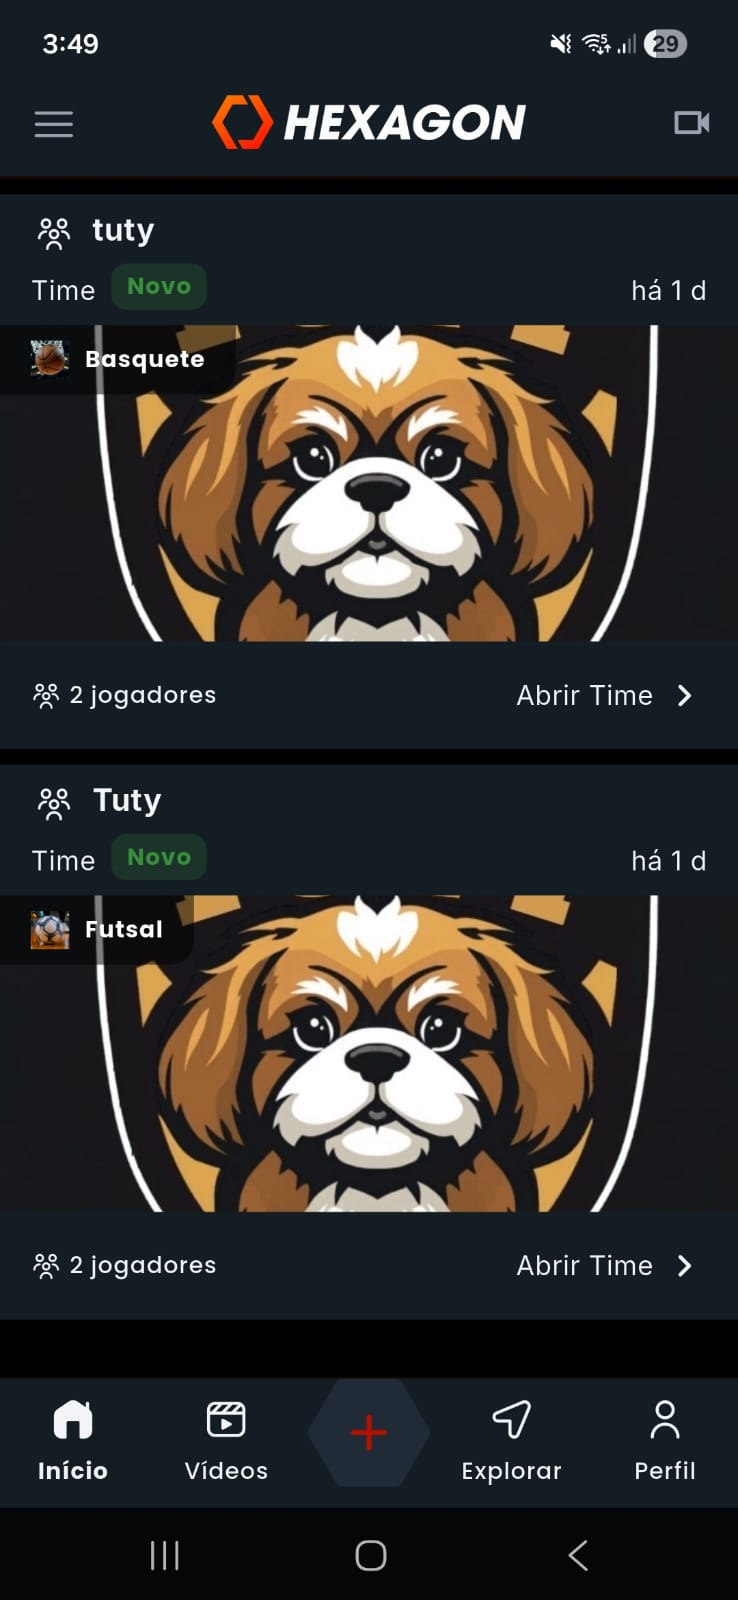
\includegraphics[width=0.95\textwidth]{assets/concorrentes/hexagon_screen_1.jpeg}
        }
        \caption*{Tela inicial}
    \end{minipage}
    \hspace{0.025\textwidth}
    \begin{minipage}{0.29\textwidth}
        \centering
        \fcolorbox{gray}{white}{
            
\includegraphics[width=0.95\textwidth]{assets/concorrentes/hexagon_screen_4.jpeg}
        }
        \caption*{Interação com usuário}
    \end{minipage}
    \hspace{0.025\textwidth}
    \begin{minipage}{0.29\textwidth}
        \centering
        \fcolorbox{gray}{white}{
            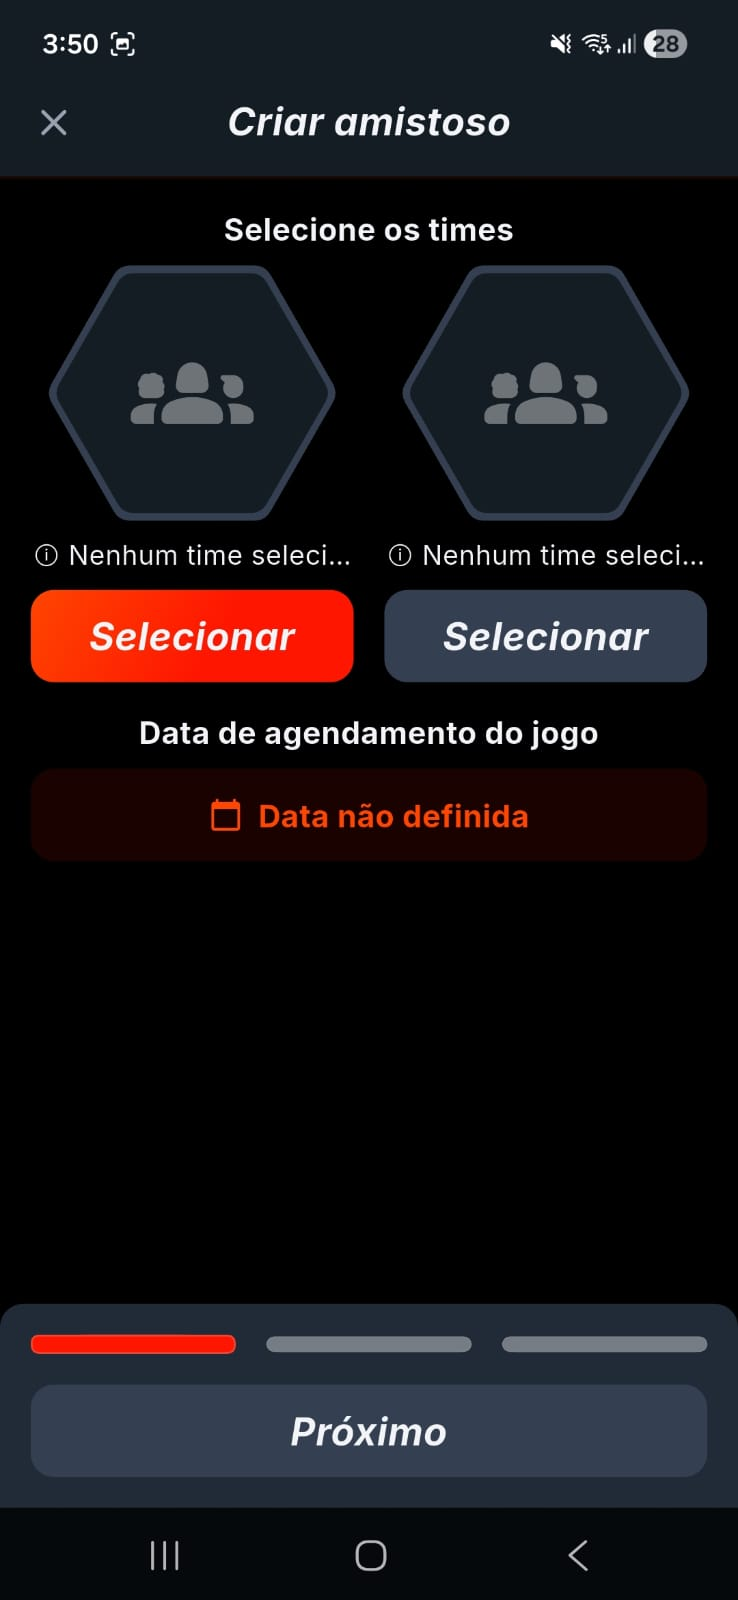
\includegraphics[width=0.95\textwidth]{assets/concorrentes/hexagon_screen_3.jpeg}
        }
        \caption*{Criação de partida}
    \end{minipage}

    \caption{Telas do Hexagon Sports utilizadas na análise comparativa}
    \label{fig:hexagon_sports_telas}
\end{figure}

\subsubsection{Meetup}

O Meetup é uma plataforma para organização de eventos e encontros presenciais de diferentes temas.\footnote{\url{https://www.meetup.com/}} Embora não seja especificamente voltado a esportes, pode ser utilizado para formar grupos de corrida, futebol, vôlei ou outras atividades coletivas.

O critério \textbf{partidas} foi classificado como \textbf{Parcial}, pois o Meetup permite a criação e participação em eventos, mas esses eventos não são necessariamente estruturados como partidas esportivas. A plataforma não oferece, de forma específica, campos como modalidade, nível da partida, número de jogadores por time, confirmação esportiva de presença ou controle de vagas voltado à prática coletiva.

O critério \textbf{grupos} foi marcado como \textbf{Sim}, já que a plataforma é fortemente baseada na criação de comunidades e grupos de interesse. Esse é um ponto relevante, pois demonstra que o Meetup resolve bem parte do problema social de reunir pessoas com interesses semelhantes.

O critério \textbf{multi-esporte} foi classificado como \textbf{Sim}, pois, por ser uma plataforma genérica, permite a criação de grupos e eventos para diferentes modalidades esportivas. Entretanto, esse suporte ocorre de maneira ampla e não especializada.

O critério \textbf{reputação} foi marcado como \textbf{Parcial}. A plataforma pode apresentar perfis de usuários, organizadores e informações sobre grupos, mas não possui, como foco principal, um mecanismo de reputação esportiva baseado em comportamento em partidas, presença, pontualidade ou respeito entre participantes.

O critério \textbf{foco social} foi classificado como \textbf{Sim}, pois a principal finalidade da plataforma é aproximar pessoas em torno de interesses comuns. Apesar disso, sua limitação para o contexto do SquadUp está no fato de não ser uma solução especializada para esportes coletivos.

\begin{figure}[H]
    \centering
    \fcolorbox{gray}{white}{
        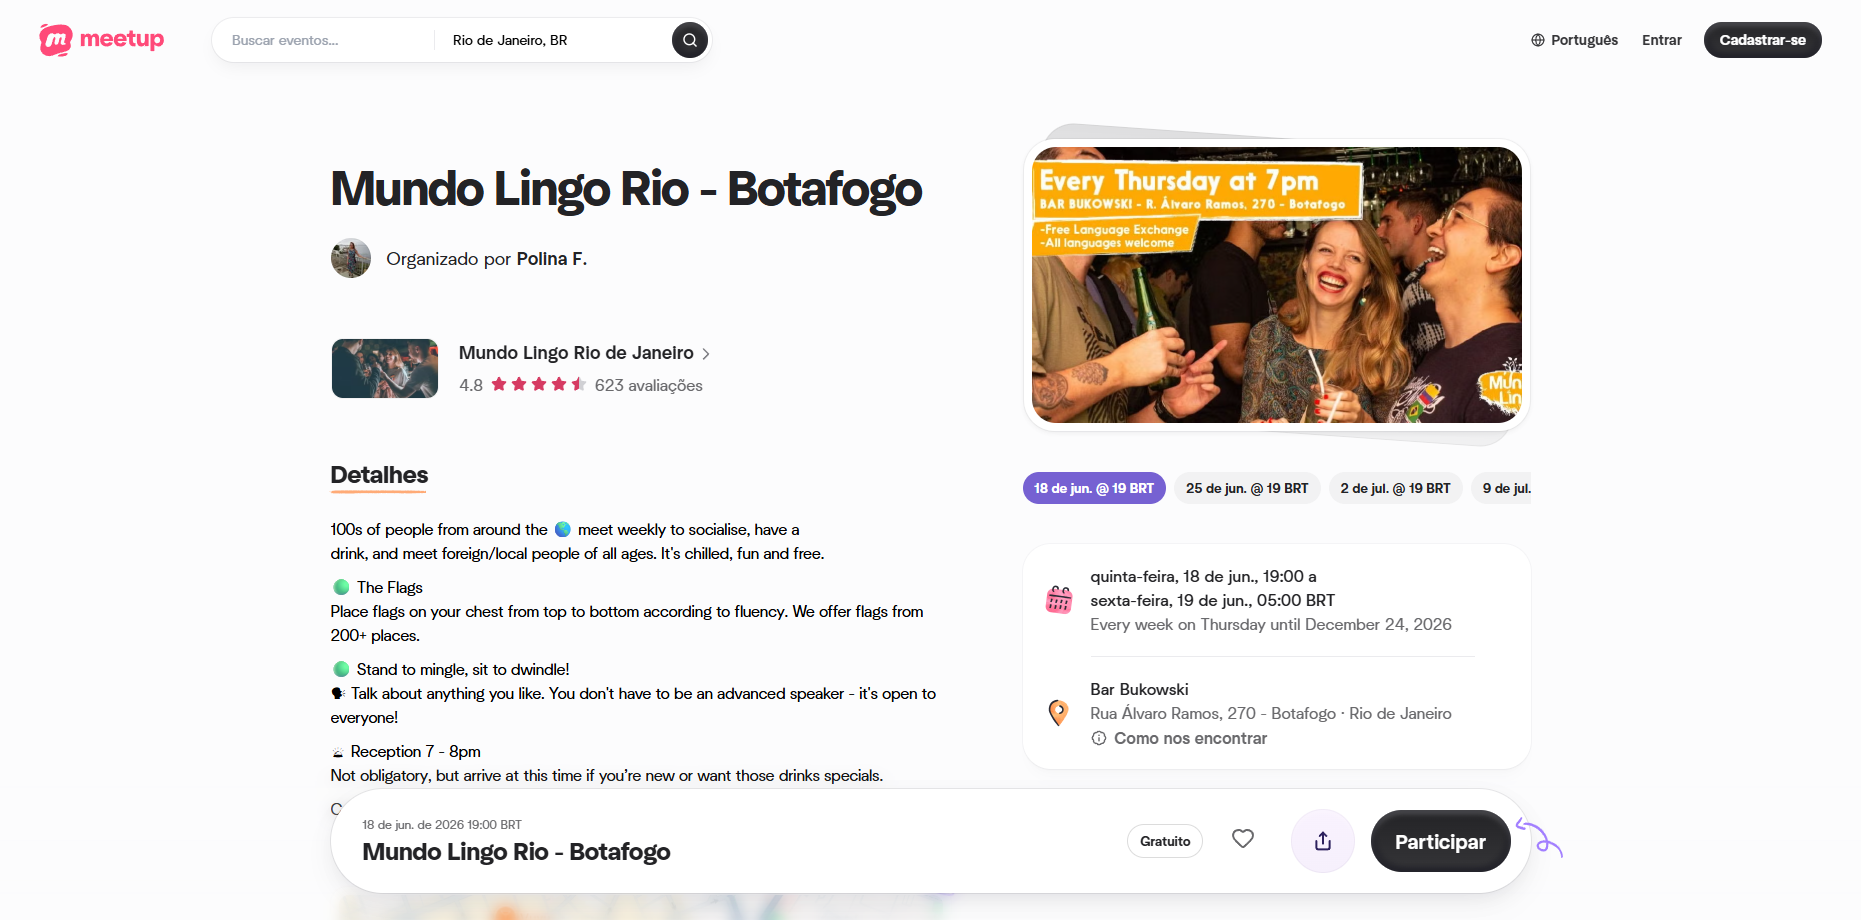
\includegraphics[width=0.9\textwidth]{assets/concorrentes/meetup_screen.png}
    }
    \caption{Tela de evento do Meetup}
    \label{fig:meetup}
\end{figure}

\subsubsection{Peladeiros}

O Peladeiros é uma aplicação voltada à organização de partidas de futebol, permitindo a criação de jogos, o controle de participantes e a comunicação entre jogadores.\footnote{\url{https://peladeiros.app}} A solução possui aderência ao problema abordado pelo SquadUp, especialmente no contexto do futebol amador.

O critério \textbf{partidas} foi classificado como \textbf{Sim}, pois a aplicação permite organizar jogos e controlar participantes. Esse aspecto está diretamente relacionado à proposta logística do SquadUp, principalmente na criação e participação em eventos esportivos.

O critério \textbf{grupos} também foi classificado como \textbf{Sim}, uma vez que a aplicação permite reunir jogadores e organizar grupos em torno das partidas. Essa funcionalidade contribui para a manutenção de comunidades esportivas já existentes.

O critério \textbf{multi-esporte}, entretanto, foi classificado como \textbf{Não}. O escopo do Peladeiros está concentrado no futebol, enquanto o SquadUp foi proposto para abranger diferentes esportes coletivos, como futebol, vôlei e basquete. Essa diferença é relevante porque o SquadUp busca atender usuários com interesses esportivos variados.

O critério \textbf{reputação} foi marcado como \textbf{Parcial}. Embora a solução possa apresentar informações sobre jogadores e participação em jogos, não foi identificado como elemento central um sistema amplo de confiança voltado à compatibilidade social, avaliação comportamental, segurança e entrada de usuários desconhecidos.

O critério \textbf{foco social} também foi classificado como \textbf{Parcial}. O Peladeiros possui um componente social, já que envolve jogadores e grupos, mas seu foco principal está na organização de partidas de futebol. O SquadUp, por outro lado, coloca a conexão social e a confiança entre usuários como elementos centrais da experiência.

\begin{figure}[H]
    \centering
    \fcolorbox{gray}{white}{
        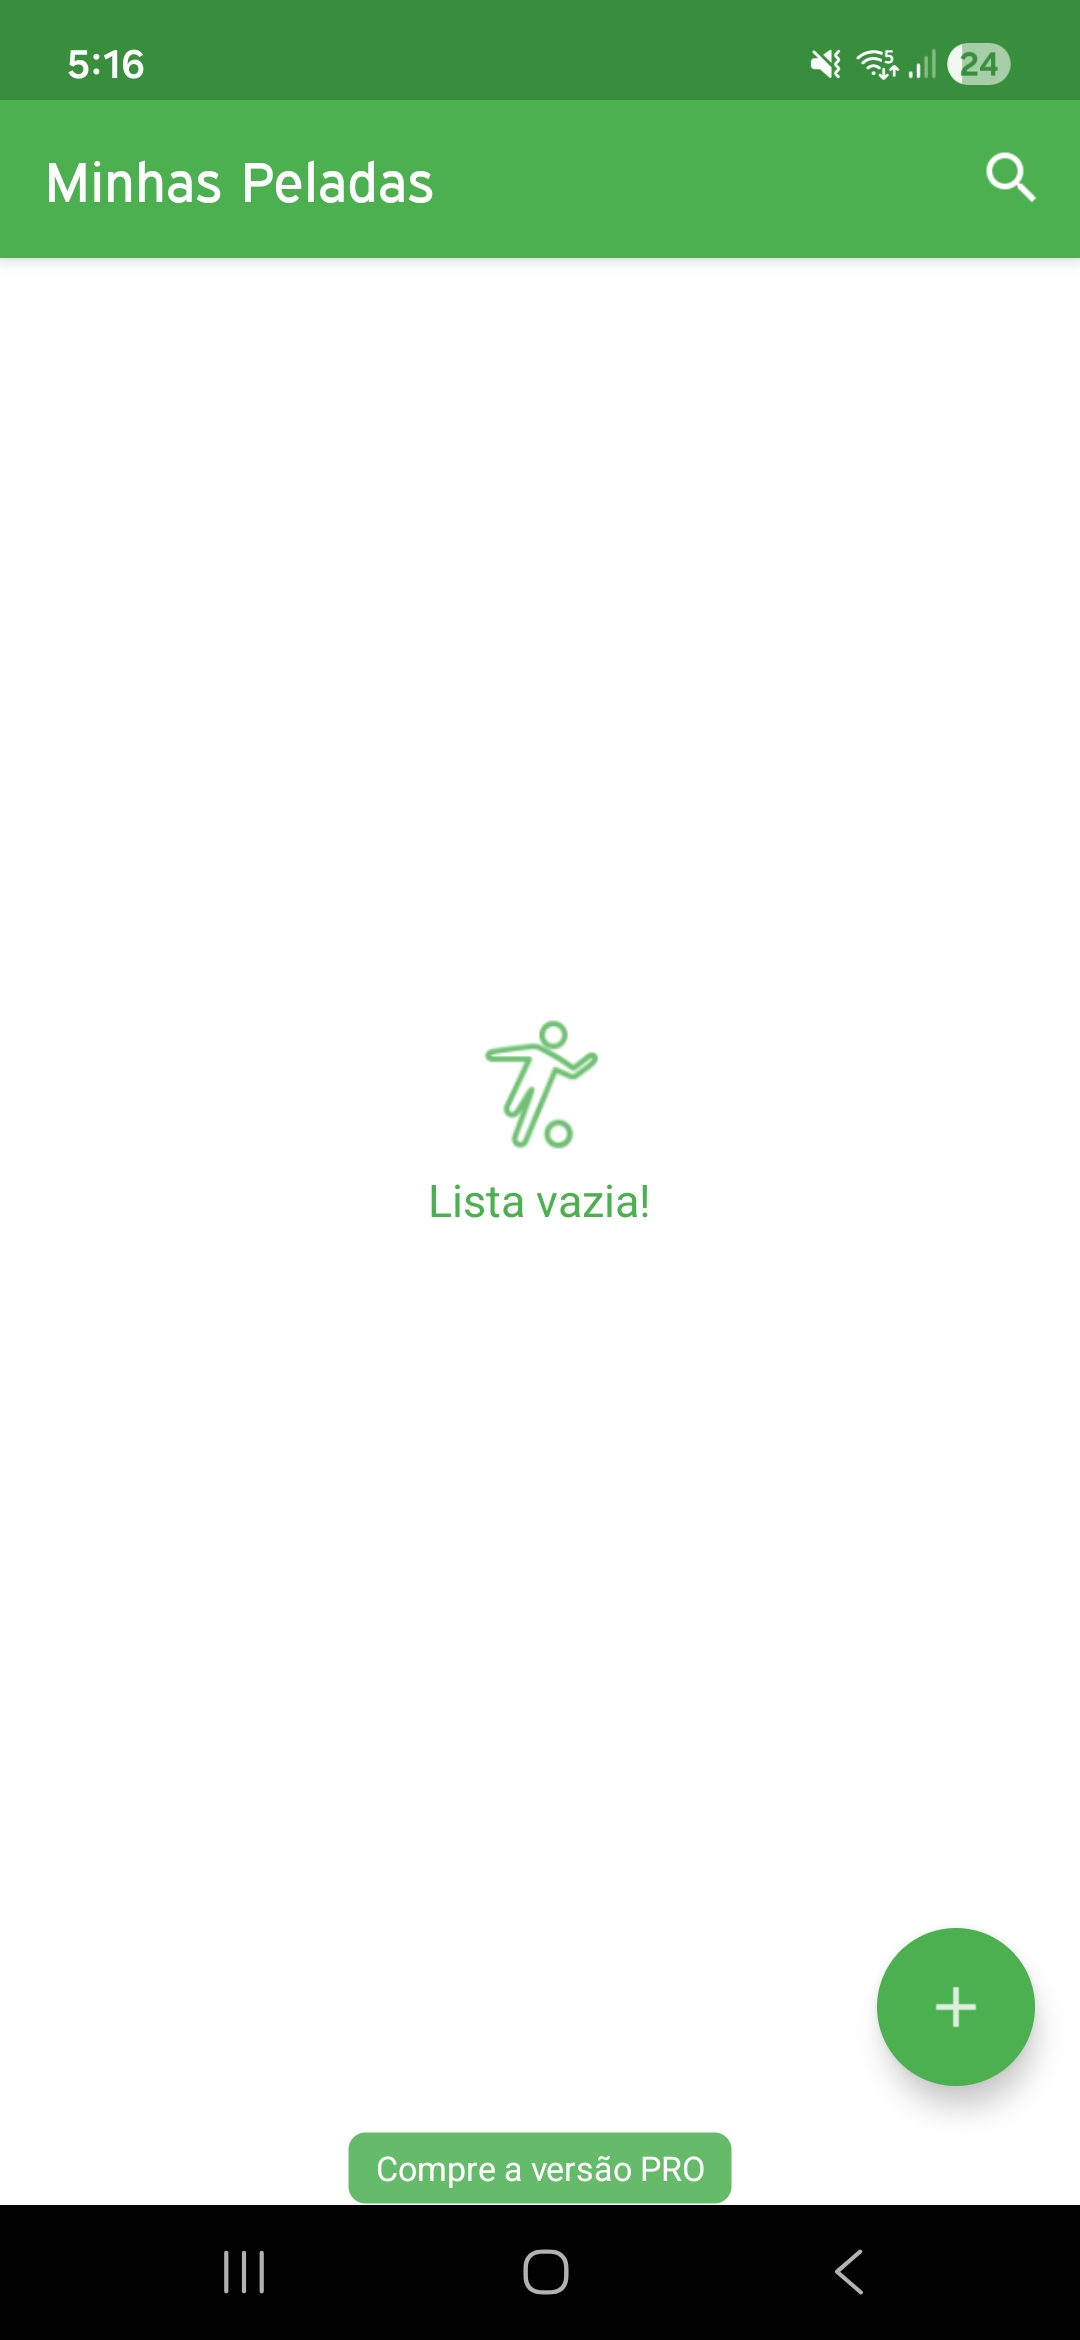
\includegraphics[width=0.32\textwidth]{assets/concorrentes/peladeiros.jpeg}
    }
    \caption{Tela inicial do Peladeiros, mostrando foco na criação de partidas de futebol}
    \label{fig:peladeiros}
\end{figure}

\subsubsection{Strava}

O Strava é uma aplicação amplamente utilizada para registro de atividades físicas, especialmente corrida e ciclismo.\footnote{\url{https://www.strava.com/}} A plataforma possui forte componente social, permitindo que usuários compartilhem atividades, acompanhem amigos e participem de desafios.

O critério \textbf{partidas} foi classificado como \textbf{Não}, pois o Strava não tem como finalidade principal criar ou organizar partidas esportivas coletivas. Seu foco está no registro de atividades físicas realizadas individualmente ou em pequenos grupos, principalmente corrida e ciclismo.

O critério \textbf{grupos} foi marcado como \textbf{Parcial}. A plataforma permite clubes, conexões entre usuários e acompanhamento de atividades de outras pessoas, mas esses grupos não são voltados especificamente à formação de partidas ou eventos coletivos com controle de participantes e vagas.

O critério \textbf{multi-esporte} foi classificado como \textbf{Parcial}. Embora o Strava permita registrar diferentes tipos de atividade física, sua proposta é mais forte em modalidades individuais, como corrida e ciclismo. Assim, o suporte a múltiplas atividades não corresponde plenamente ao conceito de múltiplos esportes coletivos abordado pelo SquadUp.

O critério \textbf{reputação} foi marcado como \textbf{Não}. A plataforma possui curtidas, comentários, seguidores e métricas de desempenho, mas esses elementos não funcionam como reputação para avaliar comportamento, presença, pontualidade ou confiabilidade de usuários em partidas.

O critério \textbf{foco social} foi classificado como \textbf{Parcial}. O Strava possui recursos sociais relevantes, mas a interação social ocorre principalmente em torno do compartilhamento de atividades já realizadas, e não da organização de encontros esportivos coletivos.

\begin{figure}[H]
    \centering
    \fcolorbox{gray}{white}{
        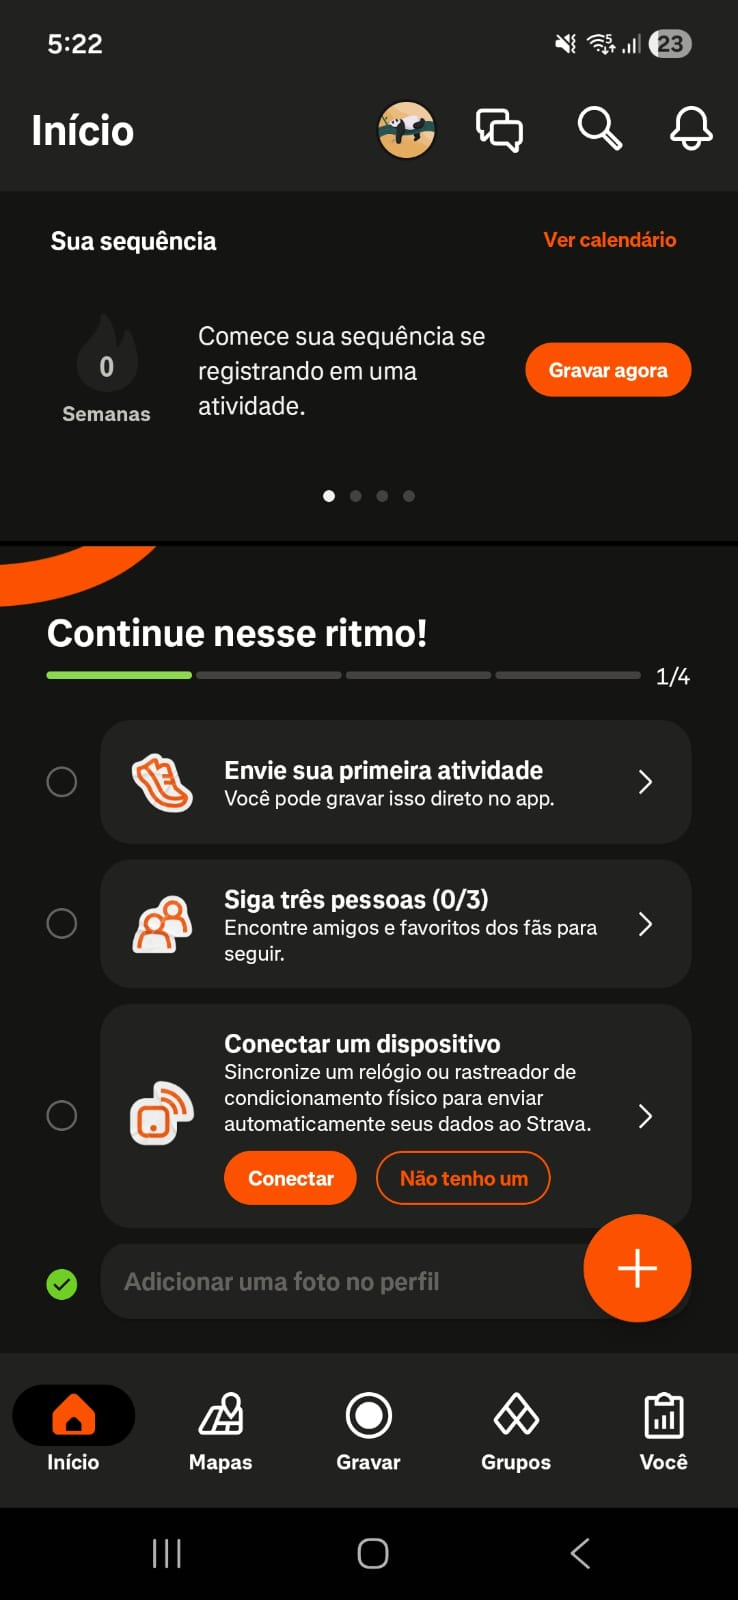
\includegraphics[width=0.32\textwidth]{assets/concorrentes/strava.jpeg}
    }
    \caption{Tela inicial do Strava}
    \label{fig:strava}
\end{figure}

\subsubsection{Grupos de WhatsApp e redes sociais}

Atualmente, muitos grupos esportivos são organizados por meio de WhatsApp, Instagram, Facebook ou outras redes sociais. Essas ferramentas são acessíveis e amplamente utilizadas, mas não foram projetadas especificamente para a organização de esportes coletivos.

O critério \textbf{partidas} foi classificado como \textbf{Parcial}, pois é possível combinar partidas por meio dessas ferramentas, mas de forma informal e pouco estruturada. Normalmente, informações como horário, local, número de vagas e presença dos participantes ficam espalhadas em mensagens, o que dificulta o acompanhamento.

O critério \textbf{grupos} foi classificado como \textbf{Sim}, já que essas plataformas permitem a criação de grupos de conversa e comunidades. Esse é um dos principais motivos pelos quais tais ferramentas são amplamente utilizadas para organização esportiva informal.

O critério \textbf{multi-esporte} foi marcado como \textbf{Sim}, pois essas ferramentas são genéricas e podem ser usadas para qualquer modalidade. No entanto, esse suporte não decorre de funcionalidades esportivas específicas, mas da flexibilidade das plataformas.

O critério \textbf{reputação} foi classificado como \textbf{Não}, pois não há mecanismos estruturados de avaliação, histórico esportivo, presença, comportamento ou validação de perfil voltados à prática de esportes coletivos.

O critério \textbf{foco social} foi marcado como \textbf{Parcial}. Embora essas ferramentas sejam sociais por natureza, seu foco não está na descoberta de novas partidas ou na entrada segura de usuários desconhecidos em grupos esportivos. Em geral, elas funcionam melhor para pessoas que já fazem parte de um círculo social ou grupo previamente formado.

\subsection{Considerações finais}

A análise da literatura e dos aplicativos relacionados indica que existem soluções voltadas à atividade física, à organização de eventos, à reserva de espaços ou ao registro de desempenho. Entretanto, poucas soluções integram, de forma equilibrada, os três pilares centrais do SquadUp: social, logístico e saúde.

A principal lacuna identificada está na conexão segura entre usuários desconhecidos para prática de esportes coletivos. Grande parte das soluções analisadas resolve aspectos isolados do problema, como encontrar partidas, registrar atividades, organizar eventos ou permitir comunicação entre pessoas já conectadas, mas não trata de forma suficientemente estruturada questões como confiança, reputação, compatibilidade entre participantes e inclusão de usuários sem grupo fixo.

Dessa forma, o SquadUp atua como uma plataforma voltada à conexão social para esportes coletivos, com apoio logístico e incentivo à continuidade da prática esportiva. O diferencial do sistema está em priorizar o pilar social e os mecanismos de confiança, sem desconsiderar os aspectos práticos necessários para que a atividade aconteça.

\clearpage

\section{Desenvolvimento Funcional do SquadUp}

Esta seção apresenta o desenvolvimento funcional do SquadUp. São descritos a visão geral do sistema, seus pilares de funcionamento, os atores envolvidos, os principais casos de uso e as telas da aplicação associadas aos fluxos centrais do sistema.

\subsection{Visão geral do sistema}

O SquadUp é um aplicativo \textit{mobile} desenvolvido para conectar usuários interessados em esportes coletivos. O sistema centraliza funcionalidades relacionadas à descoberta de partidas, criação de eventos esportivos, visualização de participantes, interação entre usuários e construção de confiança por meio de mecanismos de segurança.

A aplicação não se limita ao agendamento de partidas. Seu objetivo é oferecer um ambiente que facilite a entrada de novos participantes em grupos esportivos, especialmente quando o usuário não possui uma rede prévia de contatos. Para isso, o sistema apresenta informações claras sobre as partidas, os perfis dos participantes, o nível de experiência esperado, a quantidade de vagas disponíveis e os dados relevantes para que o usuário decida se deseja participar de determinada atividade.

\subsection{Pilares do sistema}

O SquadUp foi estruturado a partir de três pilares principais: social, logístico e saúde. Esses pilares orientam tanto a definição das funcionalidades quanto a organização da experiência do usuário.

O pilar social é o eixo central da aplicação. Ele está relacionado à conexão entre usuários, à formação de grupos, à interação entre participantes e à construção de confiança. Esse pilar contempla funcionalidades como perfil do usuário, visualização de participantes, denúncias e mecanismos de segurança associados às partidas.

O pilar logístico envolve a organização prática das partidas. Ele contempla informações como modalidade esportiva, local, data, horário, quantidade de vagas, confirmação de presença e filtros de busca. Esse pilar garante que a oportunidade esportiva seja apresentada de forma estruturada, permitindo que o usuário compreenda rapidamente se determinada partida é compatível com sua disponibilidade e interesse.

O pilar de saúde está relacionado ao incentivo à prática recorrente de atividades físicas e à promoção do bem-estar por meio dos esportes coletivos. No escopo deste trabalho, esse pilar é tratado por meio da participação em partidas e do estímulo à continuidade da prática esportiva, sem envolver métricas médicas ou acompanhamento clínico.

\subsection{Atores do sistema}

Foram identificados dois atores principais para o sistema: Usuário e Administrador. O Usuário representa a pessoa que utiliza o aplicativo para se cadastrar e autenticar-se, buscar partidas, criar eventos esportivos, visualizar detalhes de partidas, participar de atividades, conversar com demais participantes, consultar perfis de outros usuários, avaliar participantes após uma partida e realizar denúncias. Quando organiza uma partida, o próprio Usuário assume também as responsabilidades de organizador, podendo aprovar participantes pendentes e encerrar a partida. O Administrador representa o papel responsável por acompanhar denúncias e executar ações de moderação quando necessário.

Essa divisão permite separar as funcionalidades de uso cotidiano da aplicação das funcionalidades voltadas à segurança e manutenção da comunidade.

\subsection{Casos de uso}

Os casos de uso descrevem as principais interações entre os atores e o SquadUp. São contemplados os fluxos associados à autenticação, às telas principais da aplicação (busca de partidas, criação de partida, visualização de detalhes, participação, visualização de perfil), às ações complementares de organização de partidas (cancelamento de participação, aprovação de participantes e encerramento de partida), à comunicação entre participantes, à construção de reputação por meio de avaliações e aos mecanismos de segurança da comunidade (denúncia e moderação).

\subsubsection{Cadastrar-se e autenticar-se}

Este caso de uso permite que o usuário crie uma conta no sistema ou acesse uma conta já existente, condição necessária para utilizar as demais funcionalidades do SquadUp.

\textbf{Ator primário:} Usuário.

\textbf{Pré-condições:} para o cadastro, o usuário não deve possuir conta associada ao e-mail informado; para o login, o usuário deve possuir uma conta previamente cadastrada.

\textbf{Pós-condições:} o usuário passa a estar autenticado no sistema e é direcionado à tela inicial da aplicação.

\textbf{Fluxo principal (cadastro):}

\begin{enumerate}
    \item O usuário acessa a opção de cadastro a partir da tela de boas-vindas;
    \item O sistema apresenta um formulário solicitando nome, e-mail, senha e data de nascimento;
    \item O usuário informa os dados solicitados;
    \item O sistema calcula a idade do usuário a partir da data de nascimento informada;
    \item O usuário é direcionado à configuração inicial de perfil, informando esportes de interesse, nível de experiência e localização aproximada;
    \item O sistema cria a conta e autentica o usuário automaticamente.
\end{enumerate}

\textbf{Fluxo principal (login):}

\begin{enumerate}
    \item O usuário acessa a opção de login a partir da tela de boas-vindas;
    \item O usuário informa e-mail e senha cadastrados;
    \item O sistema valida as credenciais informadas;
    \item O sistema autentica o usuário e o direciona à tela inicial.
\end{enumerate}

\textbf{Fluxos alternativos:}

\begin{itemize}
    \item Caso o e-mail informado no cadastro já esteja associado a uma conta, o sistema informa o usuário e sugere realizar o login;
    \item Caso a idade calculada a partir da data de nascimento seja inferior a 18 anos, o sistema impede a conclusão do cadastro;
    \item Caso as credenciais informadas no login sejam inválidas, o sistema informa o erro sem indicar especificamente qual campo está incorreto, por motivo de segurança;
    \item Em acessos futuros, o sistema pode restaurar automaticamente a sessão do usuário a partir de uma sessão previamente autenticada, sem exigir um novo login.
\end{itemize}

\begin{figure}[H]
    \centering
    \fcolorbox{gray}{white}{
        
\includegraphics[width=0.32\textwidth]{assets/app/login.png}
    }
    \caption{Tela de login do SquadUp}
    \label{fig:app_login}
\end{figure}

% Quando o screenshot da tela de cadastro estiver disponível, descomente e ajuste o caminho abaixo.
% \begin{figure}[H]
%     \centering
%     \fcolorbox{gray}{white}{
%         
\includegraphics[width=0.32\textwidth]{assets/app/cadastro.png}
%     }
%     \caption{Tela de cadastro do SquadUp}
%     \label{fig:app_cadastro}
% \end{figure}

\subsubsection{Buscar partidas}

Este caso de uso permite que o usuário encontre partidas esportivas disponíveis de acordo com seus interesses, localização e disponibilidade.

\textbf{Ator primário:} Usuário.

\textbf{Pré-condições:} devem existir partidas cadastradas no sistema.

\textbf{Pós-condições:} o usuário visualiza uma lista de partidas disponíveis e pode selecionar uma delas para consultar mais informações.

\textbf{Fluxo principal:}

\begin{enumerate}
    \item O usuário acessa a tela inicial do aplicativo;
    \item O sistema apresenta uma lista de partidas disponíveis;
    \item O usuário visualiza informações resumidas, como modalidade, local, data, horário e quantidade de participantes;
    \item O usuário seleciona uma partida para acessar seus detalhes.
\end{enumerate}

\textbf{Fluxos alternativos:}

\begin{itemize}
    \item Caso não existam partidas disponíveis, o sistema pode informar a ausência de resultados;
    \item O usuário pode optar por criar uma nova partida.
\end{itemize}

\begin{figure}[H]
    \centering
    \fcolorbox{gray}{white}{
        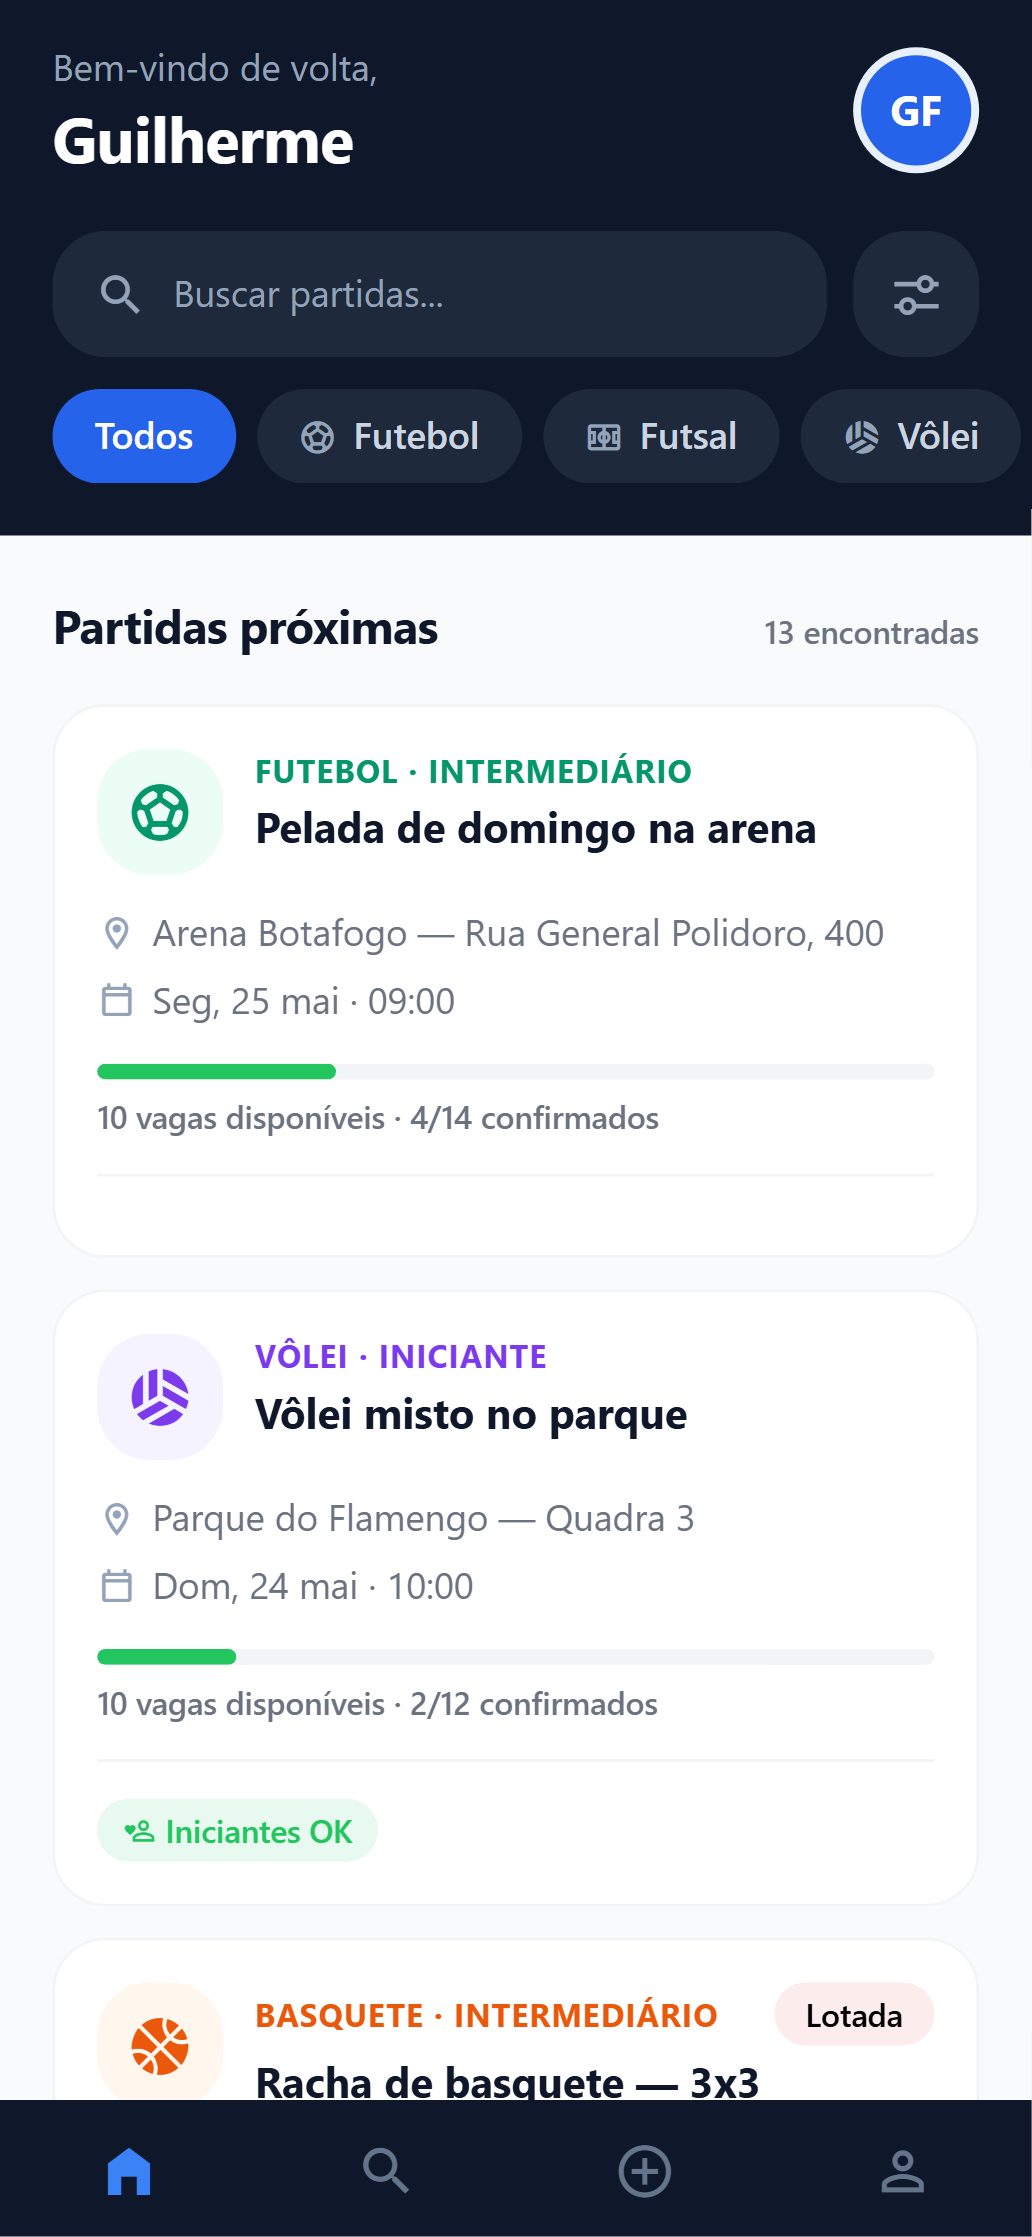
\includegraphics[width=0.32\textwidth]{assets/app/feed-principal.png}
    }
    \caption{Tela inicial do SquadUp com listagem de partidas disponíveis}
    \label{fig:app_feed_principal}
\end{figure}

\subsubsection{Criar partida}

Este caso de uso permite que um usuário organize uma nova partida esportiva, definindo suas principais informações.

\textbf{Ator primário:} Usuário.

\textbf{Pré-condições:} o usuário deve estar autenticado no sistema.

\textbf{Pós-condições:} uma nova partida é cadastrada e passa a ficar disponível para outros usuários.

\textbf{Fluxo principal:}

\begin{enumerate}
    \item O usuário acessa a opção de criação de partida;
    \item O sistema apresenta um formulário de criação;
    \item O usuário informa modalidade esportiva, título, data, horário, local, quantidade de vagas, nível da partida e descrição;
    \item O sistema valida os dados informados;
    \item O sistema cria a partida;
    \item A partida passa a ser exibida na listagem de partidas disponíveis.
\end{enumerate}

\textbf{Fluxos alternativos:}

\begin{itemize}
    \item Caso algum campo obrigatório não seja preenchido, o sistema impede a criação da partida;
    \item Caso o local informado seja inválido ou incompleto, o sistema solicita correção.
\end{itemize}

\begin{figure}[H]
    \centering
    \fcolorbox{gray}{white}{
        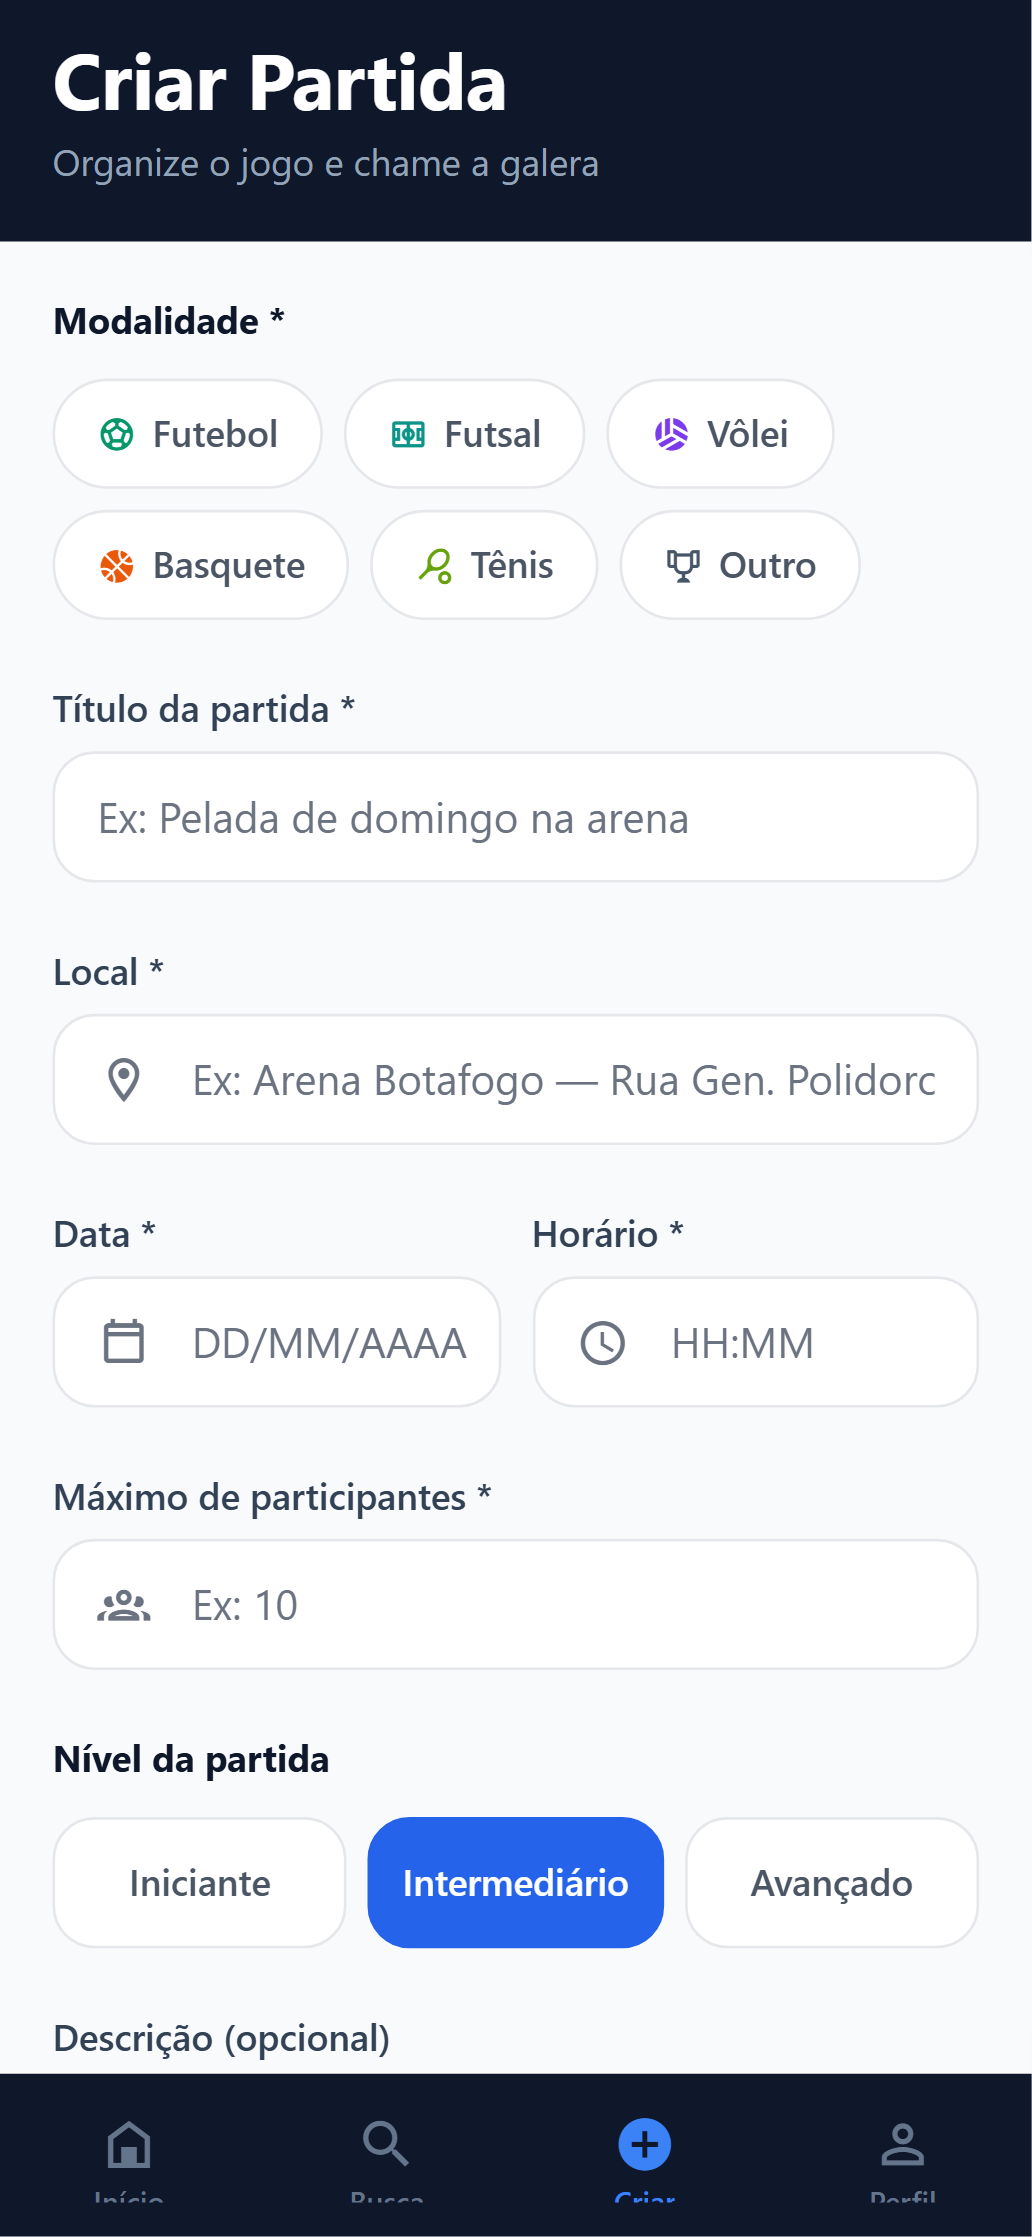
\includegraphics[width=0.32\textwidth]{assets/app/criar-partida.png}
    }
    \caption{Tela de criação de partida no SquadUp}
    \label{fig:app_criar_partida}
\end{figure}

\subsubsection{Visualizar detalhes da partida}

Este caso de uso permite que o usuário consulte as informações completas de uma partida antes de decidir participar.

\textbf{Ator primário:} Usuário.

\textbf{Pré-condições:} a partida deve estar cadastrada no sistema.

\textbf{Pós-condições:} o usuário visualiza os detalhes da partida selecionada e pode decidir se deseja participar.

\textbf{Fluxo principal:}

\begin{enumerate}
    \item O usuário seleciona uma partida na listagem;
    \item O sistema exibe informações como modalidade, data, horário, local, vagas disponíveis, nível da partida e descrição;
    \item O sistema exibe informações complementares da partida, como organizador e participantes;
    \item O usuário analisa as informações apresentadas;
    \item O usuário decide se deseja participar da partida.
\end{enumerate}

\textbf{Fluxos alternativos:}

\begin{itemize}
    \item Caso a partida esteja lotada, o sistema informa a indisponibilidade de vagas;
    \item Caso o usuário já esteja participando da partida, o sistema pode exibir essa condição na tela de detalhes.
\end{itemize}

\begin{figure}[H]
    \centering

    \begin{minipage}{0.32\textwidth}
        \centering
        \fcolorbox{gray}{white}{
            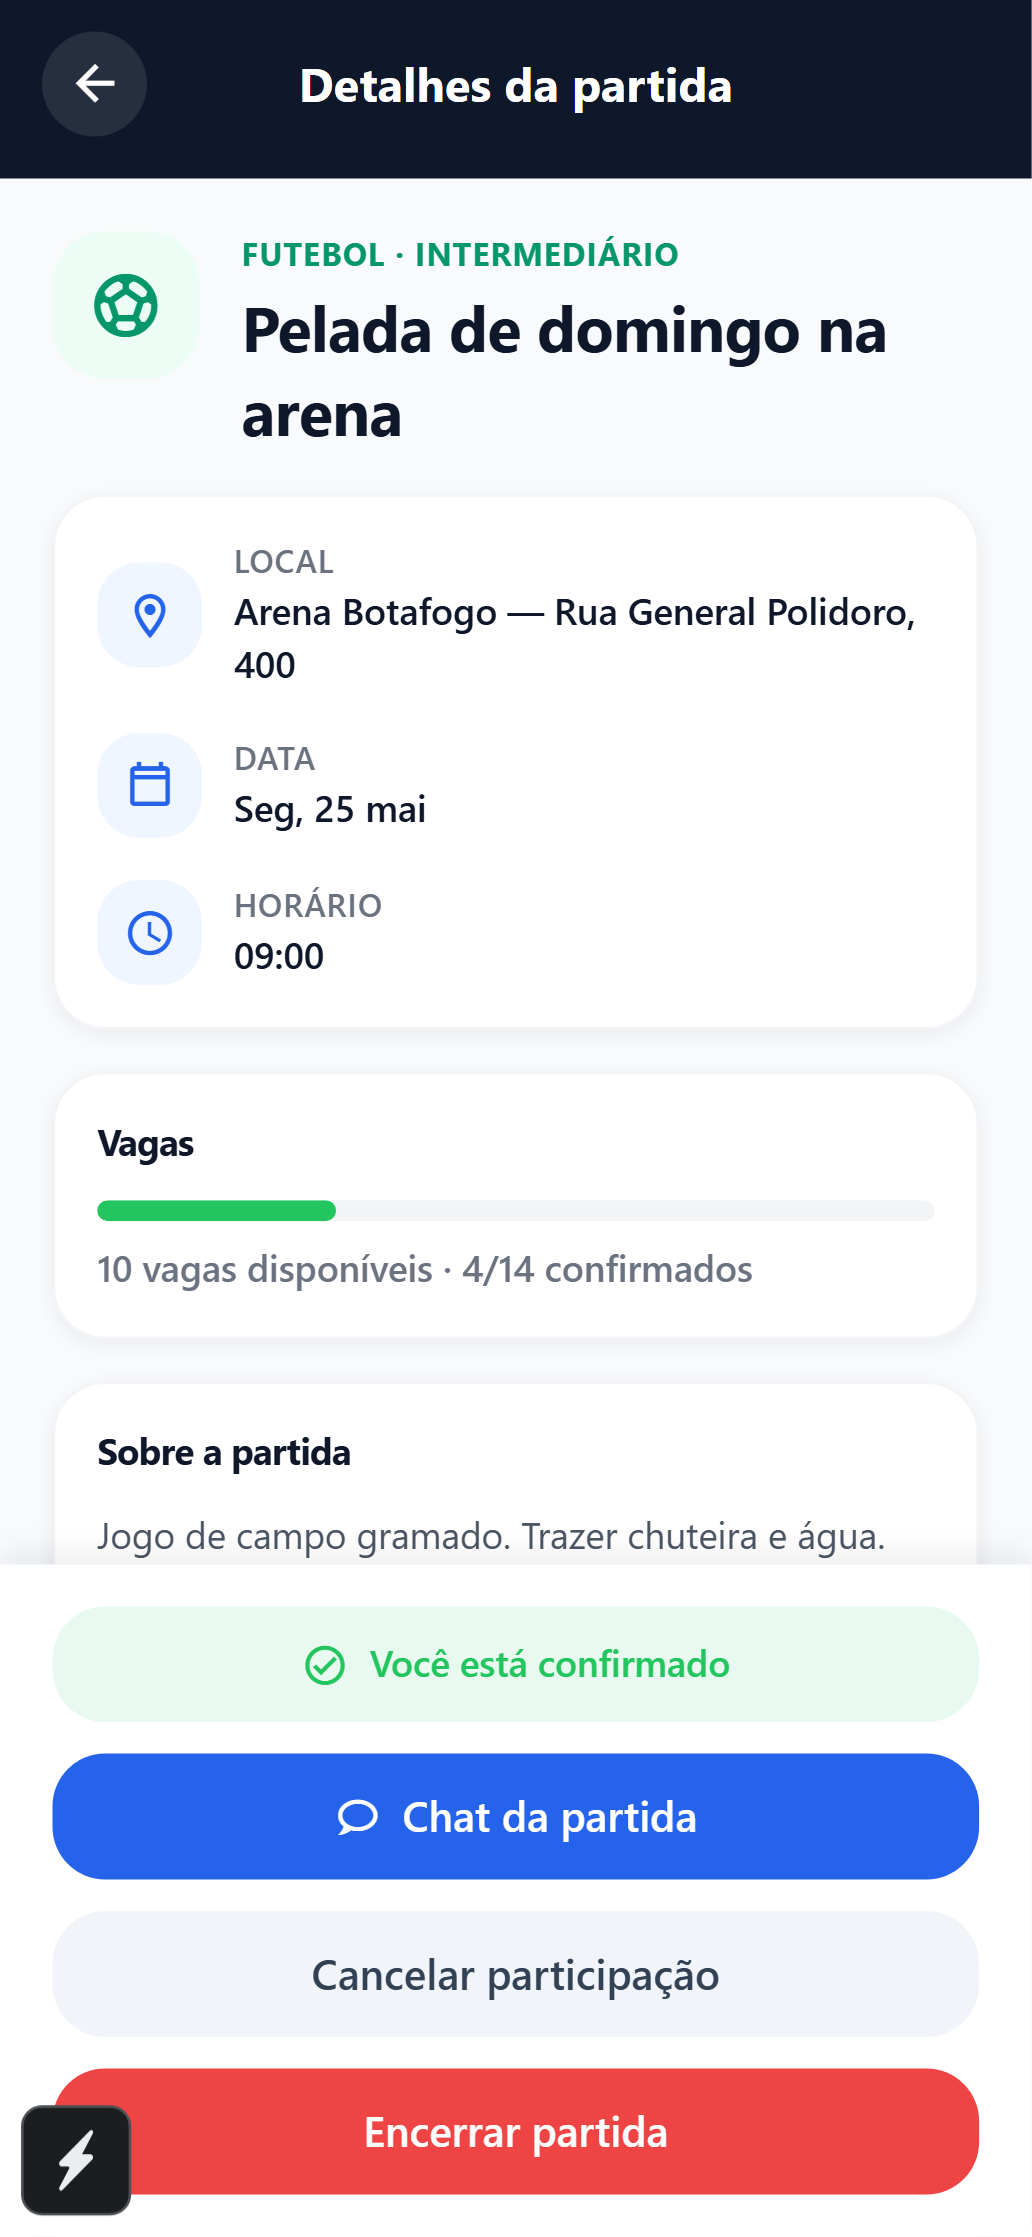
\includegraphics[width=0.95\textwidth]{assets/app/detalhes-partida.png}
        }
        \caption*{Informações gerais}
    \end{minipage}
    \hspace{0.05\textwidth}
    \begin{minipage}{0.32\textwidth}
        \centering
        \fcolorbox{gray}{white}{
            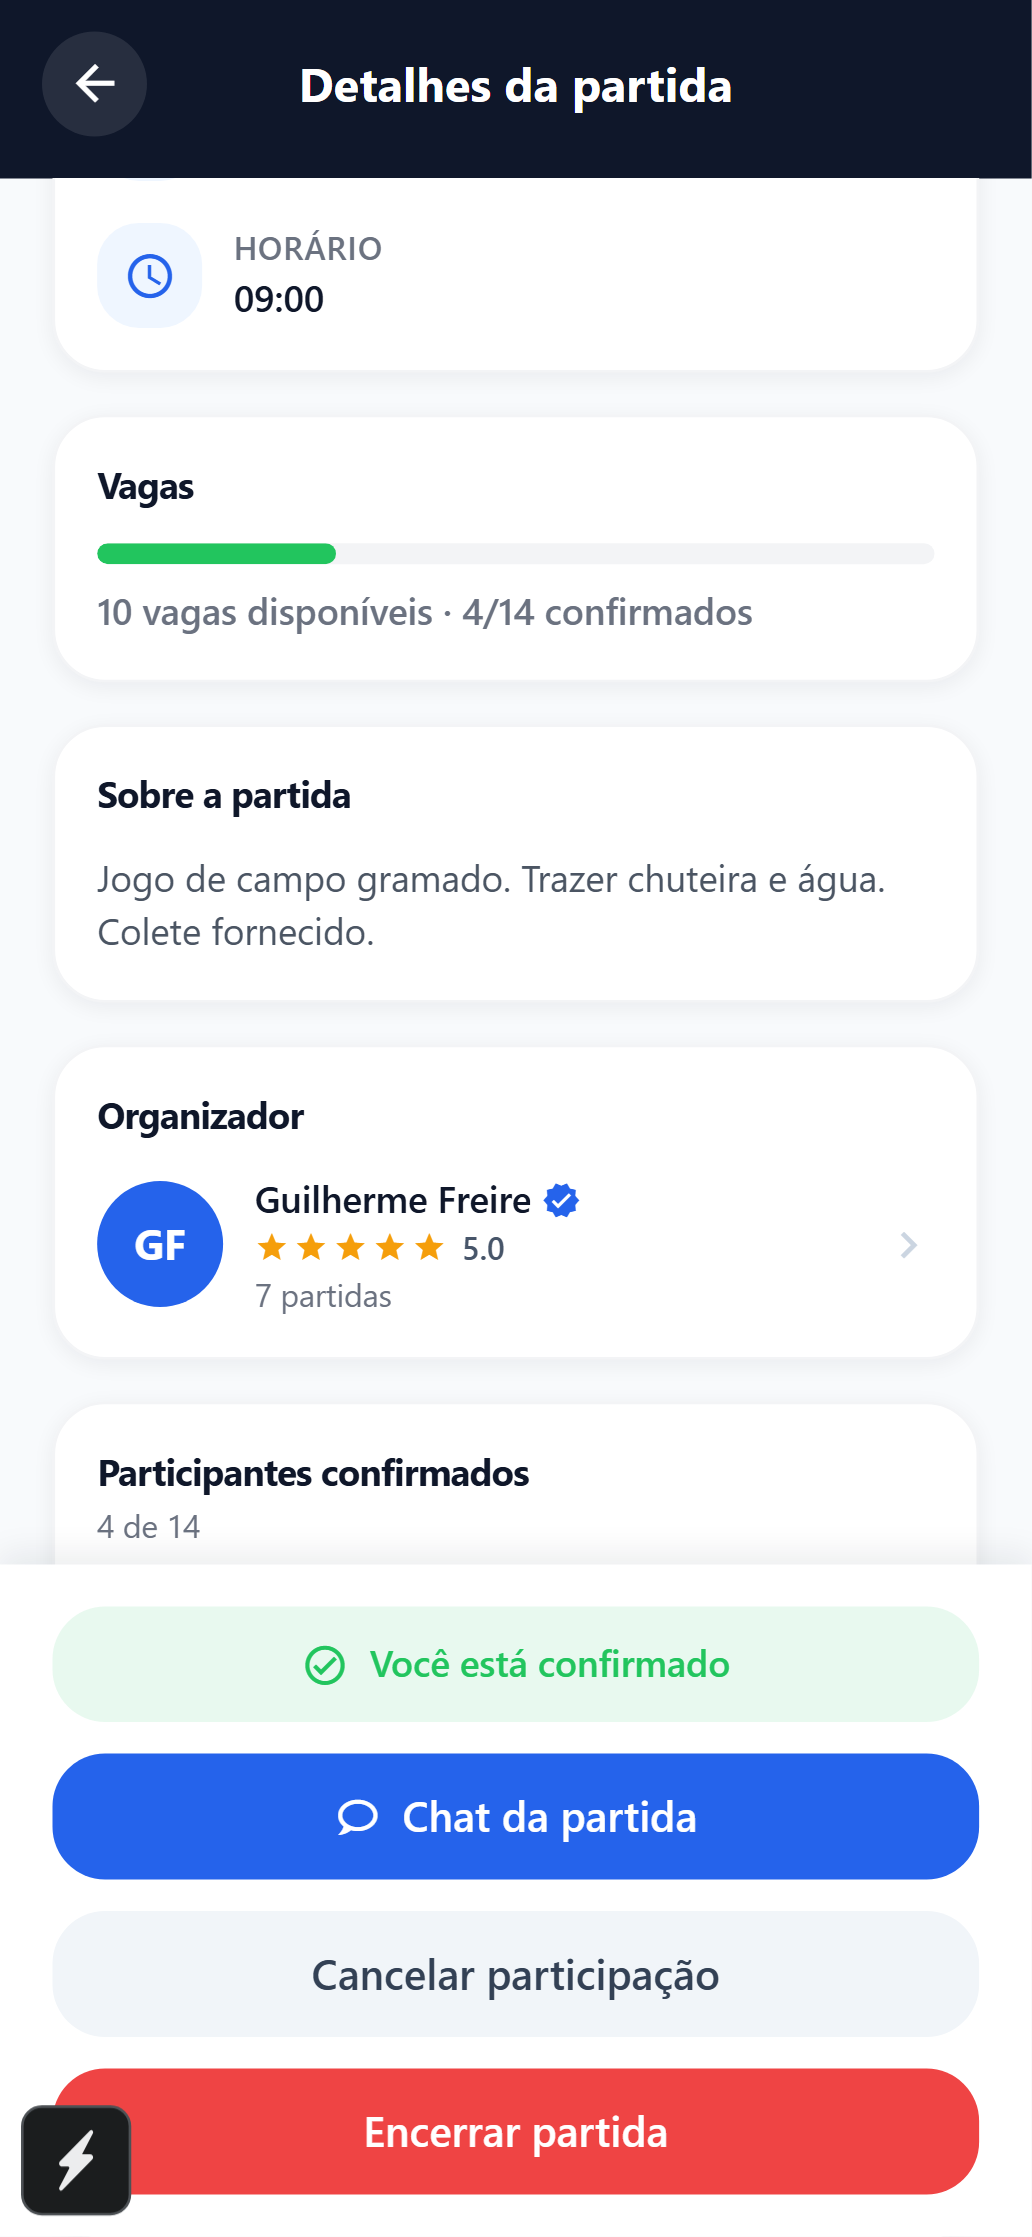
\includegraphics[width=0.95\textwidth]{assets/app/detalhes-partida-2.png}
        }
        \caption*{Informações complementares}
    \end{minipage}

    \caption{Telas de detalhes da partida no SquadUp}
    \label{fig:app_detalhes_partida}
\end{figure}

\subsubsection{Participar de partida}

Este caso de uso permite que o usuário confirme sua participação em uma partida esportiva a partir da tela de detalhes.

\textbf{Ator primário:} Usuário.

\textbf{Pré-condições:} o usuário deve estar autenticado e a partida deve possuir vagas disponíveis.

\textbf{Pós-condições:} o usuário passa a constar como participante da partida.

\textbf{Fluxo principal:}

\begin{enumerate}
    \item O usuário acessa os detalhes da partida;
    \item O sistema apresenta as informações necessárias para a decisão de participação;
    \item O usuário seleciona a opção de participar;
    \item O sistema verifica a disponibilidade de vagas;
    \item O sistema registra a participação do usuário;
    \item A partida passa a considerar o usuário como participante confirmado.
\end{enumerate}

\textbf{Fluxos alternativos:}

\begin{itemize}
    \item Caso a partida esteja lotada, o sistema informa que não há vagas disponíveis;
    \item Caso a participação dependa de aprovação, o sistema registra a solicitação como pendente.
\end{itemize}

\subsubsection{Cancelar participação}

Este caso de uso permite que o usuário desista de uma partida da qual já confirmou participação ou para a qual solicitou entrada.

\textbf{Ator primário:} Usuário.

\textbf{Pré-condições:} o usuário deve estar participando da partida, de forma confirmada ou pendente de aprovação.

\textbf{Pós-condições:} o usuário deixa de constar como participante da partida, e a vaga correspondente volta a ficar disponível.

\textbf{Fluxo principal:}

\begin{enumerate}
    \item O usuário acessa os detalhes de uma partida da qual participa;
    \item O sistema exibe a opção de cancelar participação;
    \item O usuário seleciona a opção de cancelamento;
    \item O sistema solicita confirmação da ação;
    \item O sistema remove o usuário da lista de participantes da partida;
    \item A partida volta a apresentar a vaga como disponível.
\end{enumerate}

\textbf{Fluxos alternativos:}

\begin{itemize}
    \item Caso o usuário decida não confirmar a ação, o cancelamento é interrompido e a participação é mantida;
    \item Caso a partida já tenha sido encerrada, o sistema não permite o cancelamento.
\end{itemize}

\subsubsection{Aprovar participante pendente}

Este caso de uso permite que o organizador de uma partida analise e aprove solicitações de participação, aplicável a partidas configuradas para exigir aprovação manual.

\textbf{Ator primário:} Usuário (na qualidade de organizador da partida).

\textbf{Pré-condições:} o usuário deve ser o organizador da partida e deve existir ao menos uma solicitação de participação pendente.

\textbf{Pós-condições:} o participante aprovado passa a constar como confirmado na partida.

\textbf{Fluxo principal:}

\begin{enumerate}
    \item O organizador acessa os detalhes da partida que criou;
    \item O sistema exibe a lista de participantes com solicitações pendentes;
    \item O organizador seleciona a opção de aprovar um participante;
    \item O sistema verifica a disponibilidade de vagas na partida;
    \item O sistema altera o status do participante para confirmado.
\end{enumerate}

\textbf{Fluxos alternativos:}

\begin{itemize}
    \item Caso as vagas da partida já tenham sido preenchidas, o sistema impede a aprovação de novos participantes;
    \item Caso o usuário autenticado não seja o organizador da partida, o sistema não disponibiliza essa ação.
\end{itemize}

\subsubsection{Encerrar partida}

Este caso de uso permite que o organizador finalize uma partida, sinalizando que o evento já ocorreu e habilitando a avaliação entre os participantes.

\textbf{Ator primário:} Usuário (na qualidade de organizador da partida).

\textbf{Pré-condições:} o usuário deve ser o organizador da partida, e a partida não deve estar previamente encerrada.

\textbf{Pós-condições:} a partida passa a ter status encerrado, deixando de aceitar novas participações e habilitando a avaliação dos participantes.

\textbf{Fluxo principal:}

\begin{enumerate}
    \item O organizador acessa os detalhes da partida que criou;
    \item O sistema exibe a opção de encerrar a partida;
    \item O organizador seleciona a opção de encerramento;
    \item O sistema altera o status da partida para encerrado;
    \item A partida passa a habilitar a avaliação dos participantes confirmados.
\end{enumerate}

\textbf{Fluxos alternativos:}

\begin{itemize}
    \item Caso o usuário autenticado não seja o organizador da partida, o sistema não disponibiliza essa ação;
    \item Caso a partida já esteja encerrada, o sistema não permite um novo encerramento.
\end{itemize}

\subsubsection{Conversar no chat da partida}

Este caso de uso permite que participantes de uma partida troquem mensagens entre si, fortalecendo a comunicação e a coordenação antes do encontro presencial.

\textbf{Ator primário:} Usuário.

\textbf{Pré-condições:} o usuário deve ser o organizador da partida ou um participante com participação confirmada.

\textbf{Pós-condições:} a mensagem enviada passa a ficar disponível para os demais participantes da partida.

\textbf{Fluxo principal:}

\begin{enumerate}
    \item O usuário acessa o chat de uma partida da qual participa;
    \item O sistema exibe o histórico de mensagens trocadas entre os participantes;
    \item O usuário redige e envia uma nova mensagem;
    \item O sistema registra a mensagem e a distribui aos demais participantes;
    \item Os demais participantes confirmados recebem uma notificação sobre a nova mensagem.
\end{enumerate}

\textbf{Fluxos alternativos:}

\begin{itemize}
    \item Caso o usuário não seja organizador nem participante confirmado da partida, o sistema não permite o acesso ao chat;
    \item Caso o usuário negue a permissão de notificações, o recebimento de novas mensagens continua ocorrendo normalmente, sem o aviso do sistema operacional.
\end{itemize}

\begin{figure}[H]
    \centering
    \fcolorbox{gray}{white}{
        
\includegraphics[width=0.32\textwidth]{assets/app/chat-partida.png}
    }
    \caption{Tela de chat da partida no SquadUp}
    \label{fig:app_chat_partida}
\end{figure}

\subsubsection{Visualizar perfil do usuário}

Este caso de uso permite que um usuário consulte informações públicas de outro participante, contribuindo para a percepção de confiança antes da interação presencial.

\textbf{Ator primário:} Usuário.

\textbf{Pré-condições:} o perfil consultado deve estar cadastrado no sistema.

\textbf{Pós-condições:} o usuário visualiza informações públicas do participante consultado.

\textbf{Fluxo principal:}

\begin{enumerate}
    \item O usuário acessa o perfil de outro participante;
    \item O sistema exibe informações públicas, como nome, foto, esportes de interesse e informações esportivas;
    \item O usuário utiliza essas informações para avaliar a compatibilidade e a segurança da interação;
    \item O usuário pode retornar à partida ou acessar outras opções disponíveis no perfil.
\end{enumerate}

\textbf{Fluxos alternativos:}

\begin{itemize}
    \item Caso o perfil não esteja disponível, o sistema informa que não foi possível carregar os dados;
    \item Caso o usuário identifique comportamento inadequado, pode acessar o fluxo de denúncia.
\end{itemize}

\begin{figure}[H]
    \centering
    \fcolorbox{gray}{white}{
        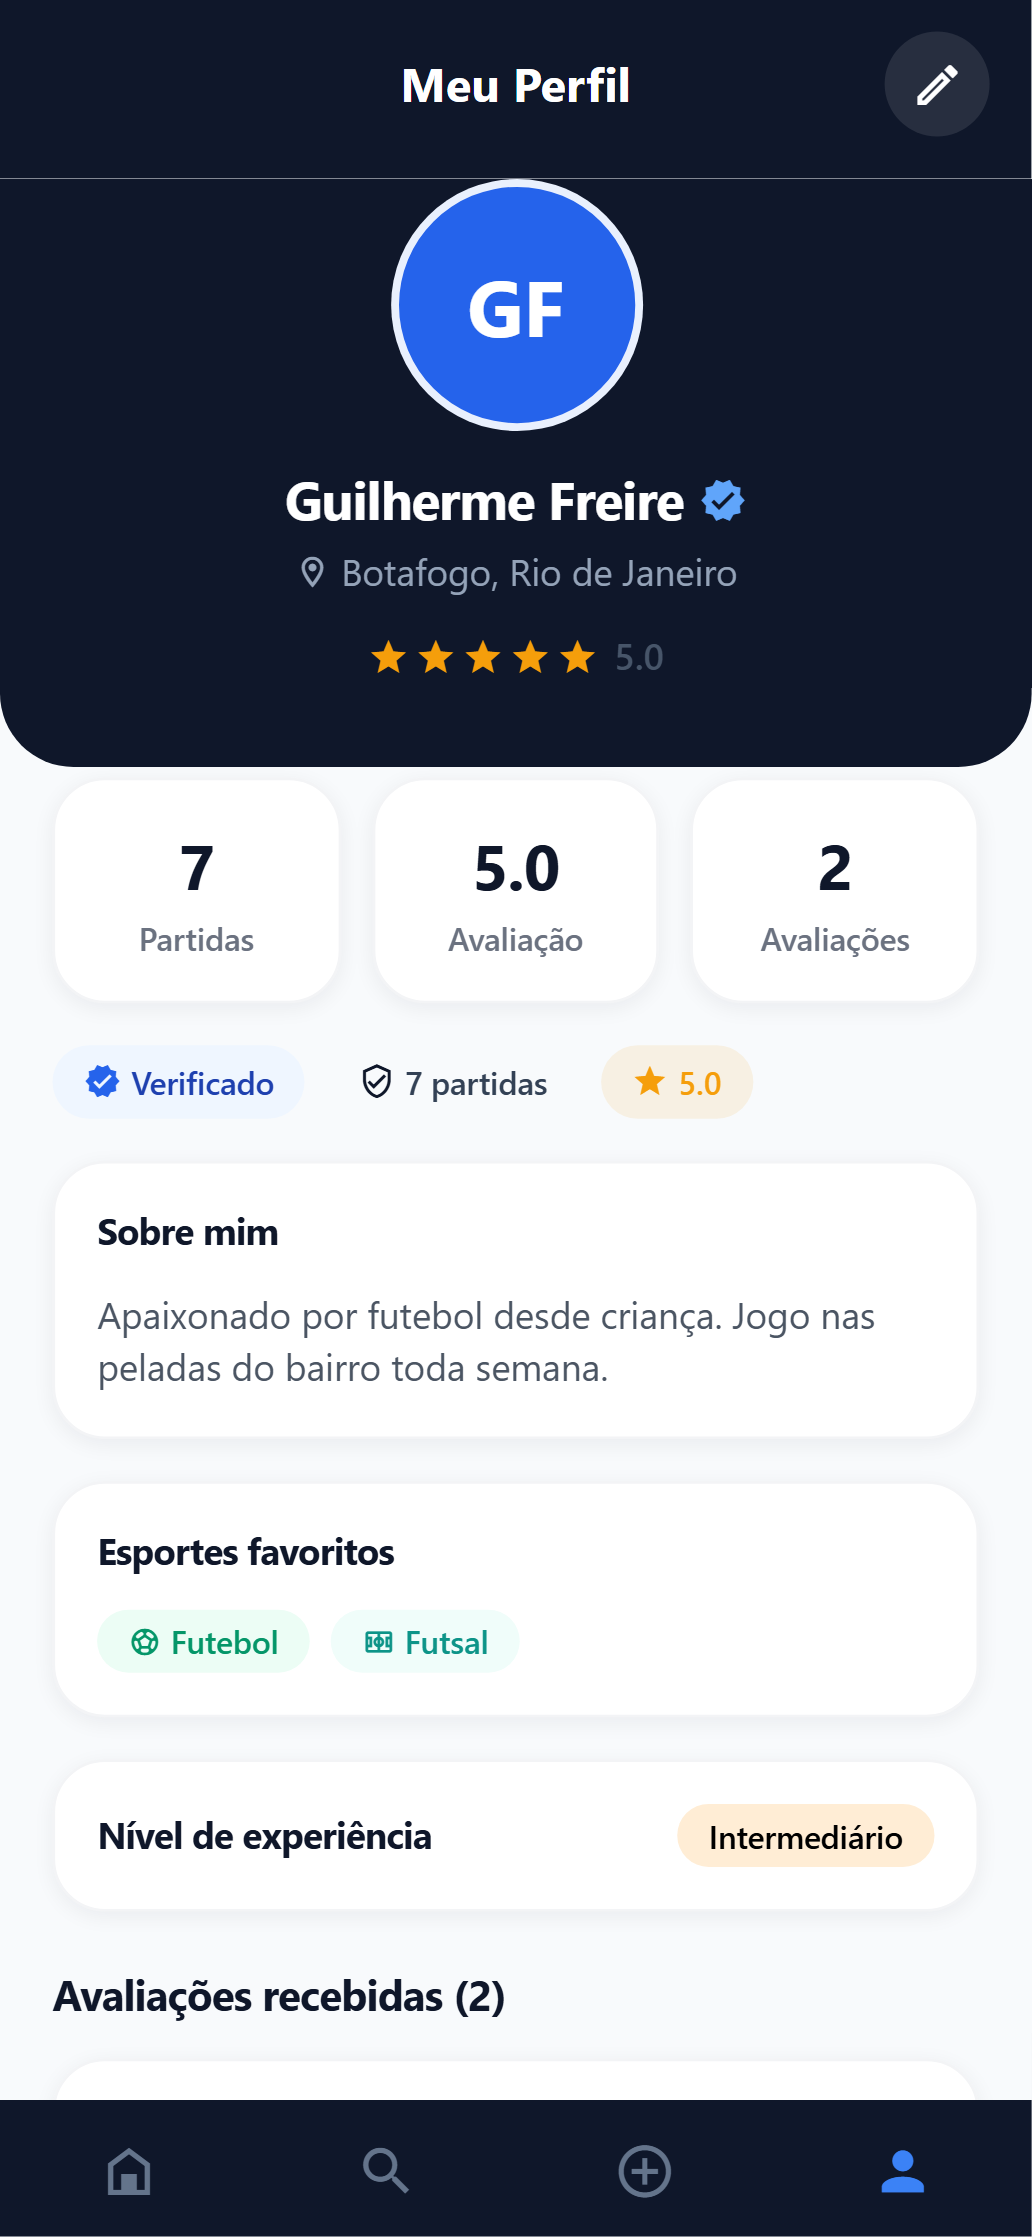
\includegraphics[width=0.32\textwidth]{assets/app/perfil.png}
    }
    \caption{Tela de perfil de usuário no SquadUp}
    \label{fig:app_perfil_usuario}
\end{figure}

\subsubsection{Avaliar usuário pós-partida}

Este caso de uso permite que participantes avaliem uns aos outros após o encerramento de uma partida, contribuindo para a construção da reputação dos usuários dentro da comunidade.

\textbf{Ator primário:} Usuário.

\textbf{Pré-condições:} a partida deve estar encerrada, e tanto o avaliador quanto o usuário avaliado devem ter participação confirmada nessa partida.

\textbf{Pós-condições:} a avaliação é registrada e passa a compor a nota média do usuário avaliado.

\textbf{Fluxo principal:}

\begin{enumerate}
    \item Após o encerramento de uma partida, o usuário acessa a lista de participantes disponíveis para avaliação;
    \item O usuário seleciona um participante a ser avaliado;
    \item O sistema apresenta um formulário com critérios de avaliação: pontualidade, respeito, comportamento, presença e experiência geral;
    \item O usuário atribui uma nota a cada critério e, opcionalmente, escreve um comentário;
    \item O usuário confirma o envio da avaliação;
    \item O sistema registra a avaliação e atualiza a reputação do usuário avaliado.
\end{enumerate}

\textbf{Fluxos alternativos:}

\begin{itemize}
    \item Caso algum critério de avaliação não seja preenchido, o sistema impede o envio da avaliação;
    \item Caso o usuário já tenha avaliado determinado participante naquela partida, o sistema indica que a avaliação já foi realizada;
    \item Caso o avaliador ou o avaliado não tenham participação confirmada na partida, o sistema não permite a avaliação.
\end{itemize}

% Quando o screenshot da tela de avaliação estiver disponível, descomente e ajuste o caminho abaixo.
% \begin{figure}[H]
%     \centering
%     \fcolorbox{gray}{white}{
%         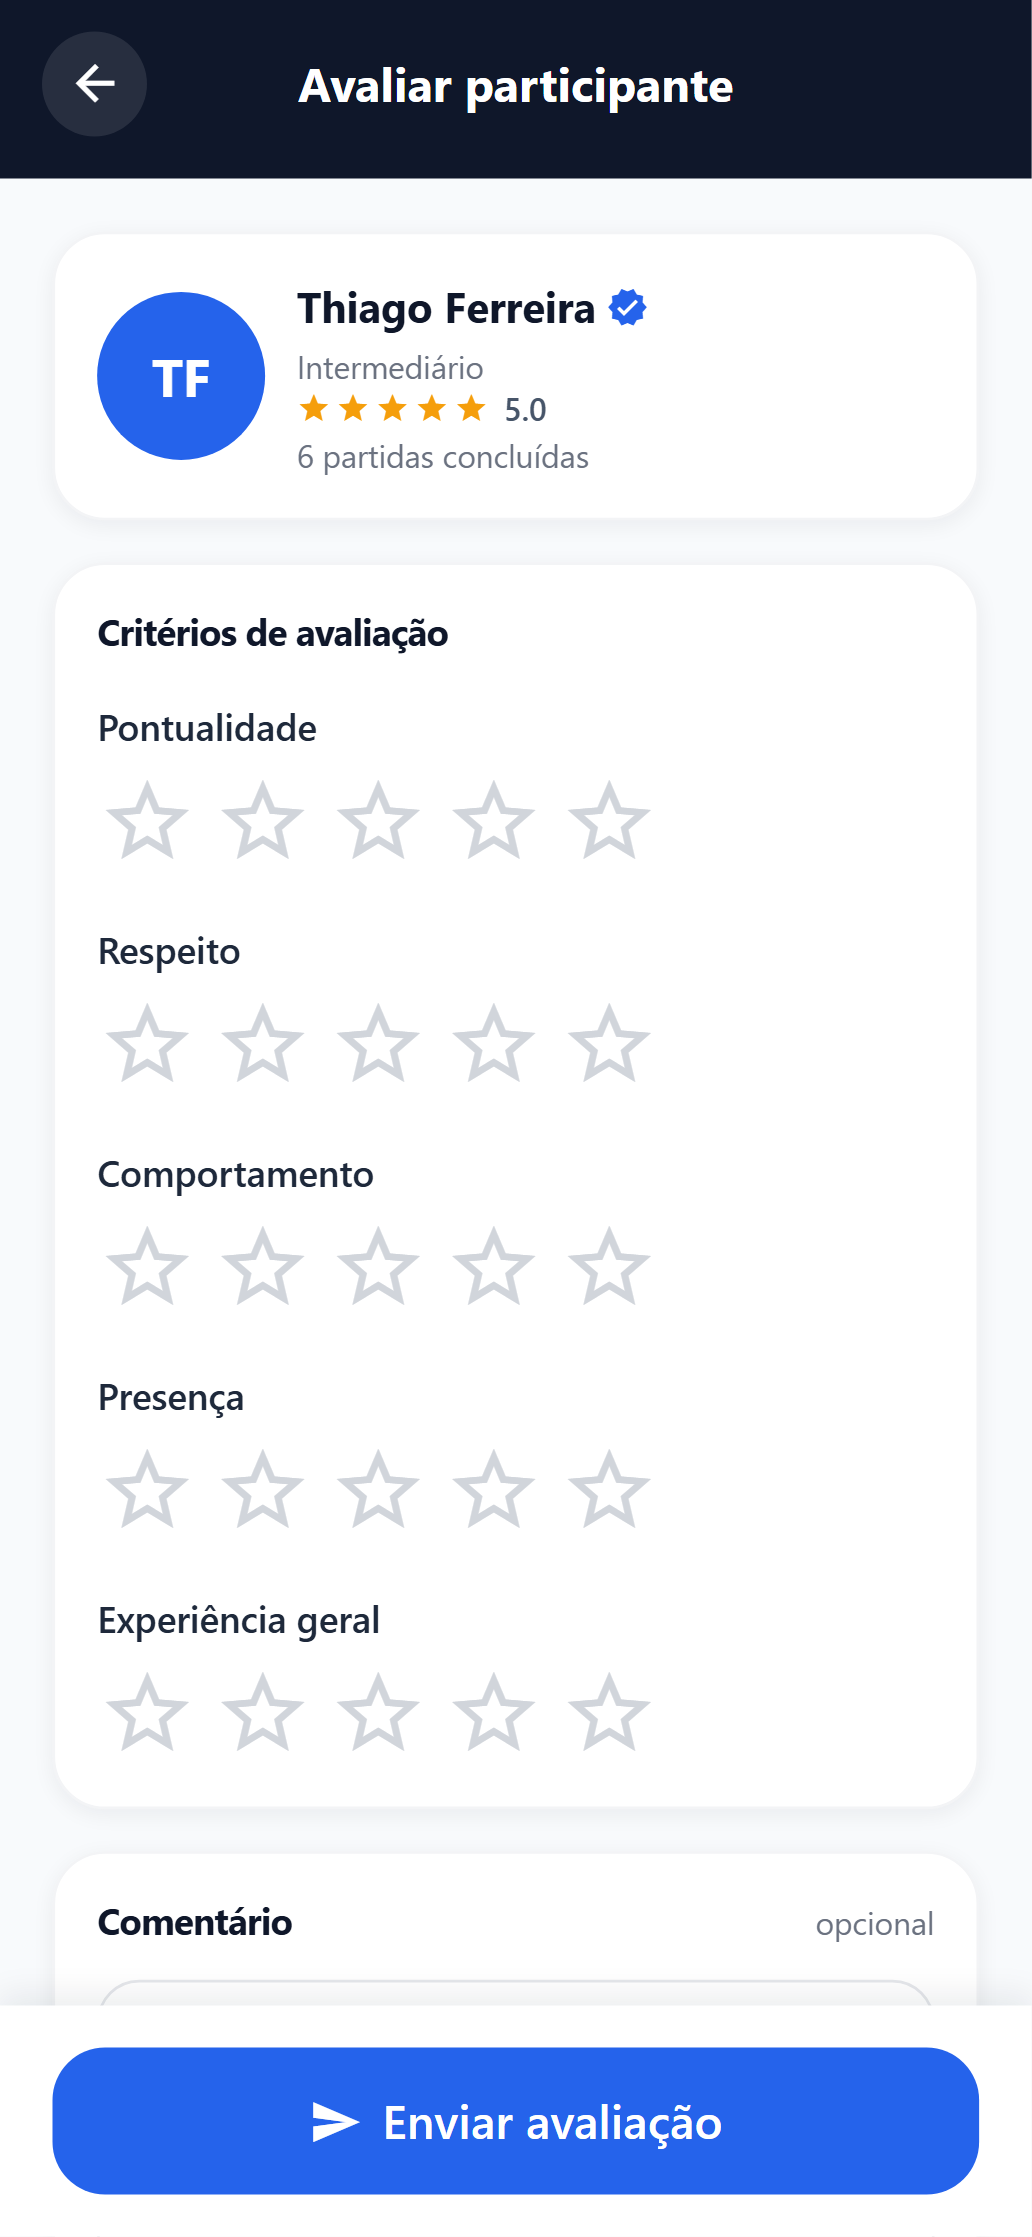
\includegraphics[width=0.32\textwidth]{assets/app/avaliacao.png}
%     }
%     \caption{Tela de avaliação pós-partida no SquadUp}
%     \label{fig:app_avaliacao}
% \end{figure}

\subsubsection{Denunciar usuário}

Este caso de uso permite que usuários reportem comportamentos inadequados, contribuindo para a segurança da comunidade.

\textbf{Ator primário:} Usuário.

\textbf{Pré-condições:} o usuário deve estar autenticado no sistema.

\textbf{Pós-condições:} uma denúncia é registrada para análise administrativa.

\textbf{Fluxo principal:}

\begin{enumerate}
    \item O usuário acessa o perfil de outro usuário ou uma opção de denúncia associada à interação;
    \item O usuário seleciona a opção de denúncia;
    \item O sistema apresenta um formulário com motivo e descrição;
    \item O usuário preenche as informações solicitadas;
    \item O sistema registra a denúncia;
    \item A denúncia fica disponível para análise administrativa.
\end{enumerate}

\textbf{Fluxos alternativos:}

\begin{itemize}
    \item Caso a denúncia esteja incompleta, o sistema solicita o preenchimento dos campos obrigatórios;
    \item Caso a denúncia seja considerada inválida, ela poderá ser encerrada sem ação administrativa.
\end{itemize}

\begin{figure}[H]
    \centering
    \fcolorbox{gray}{white}{
        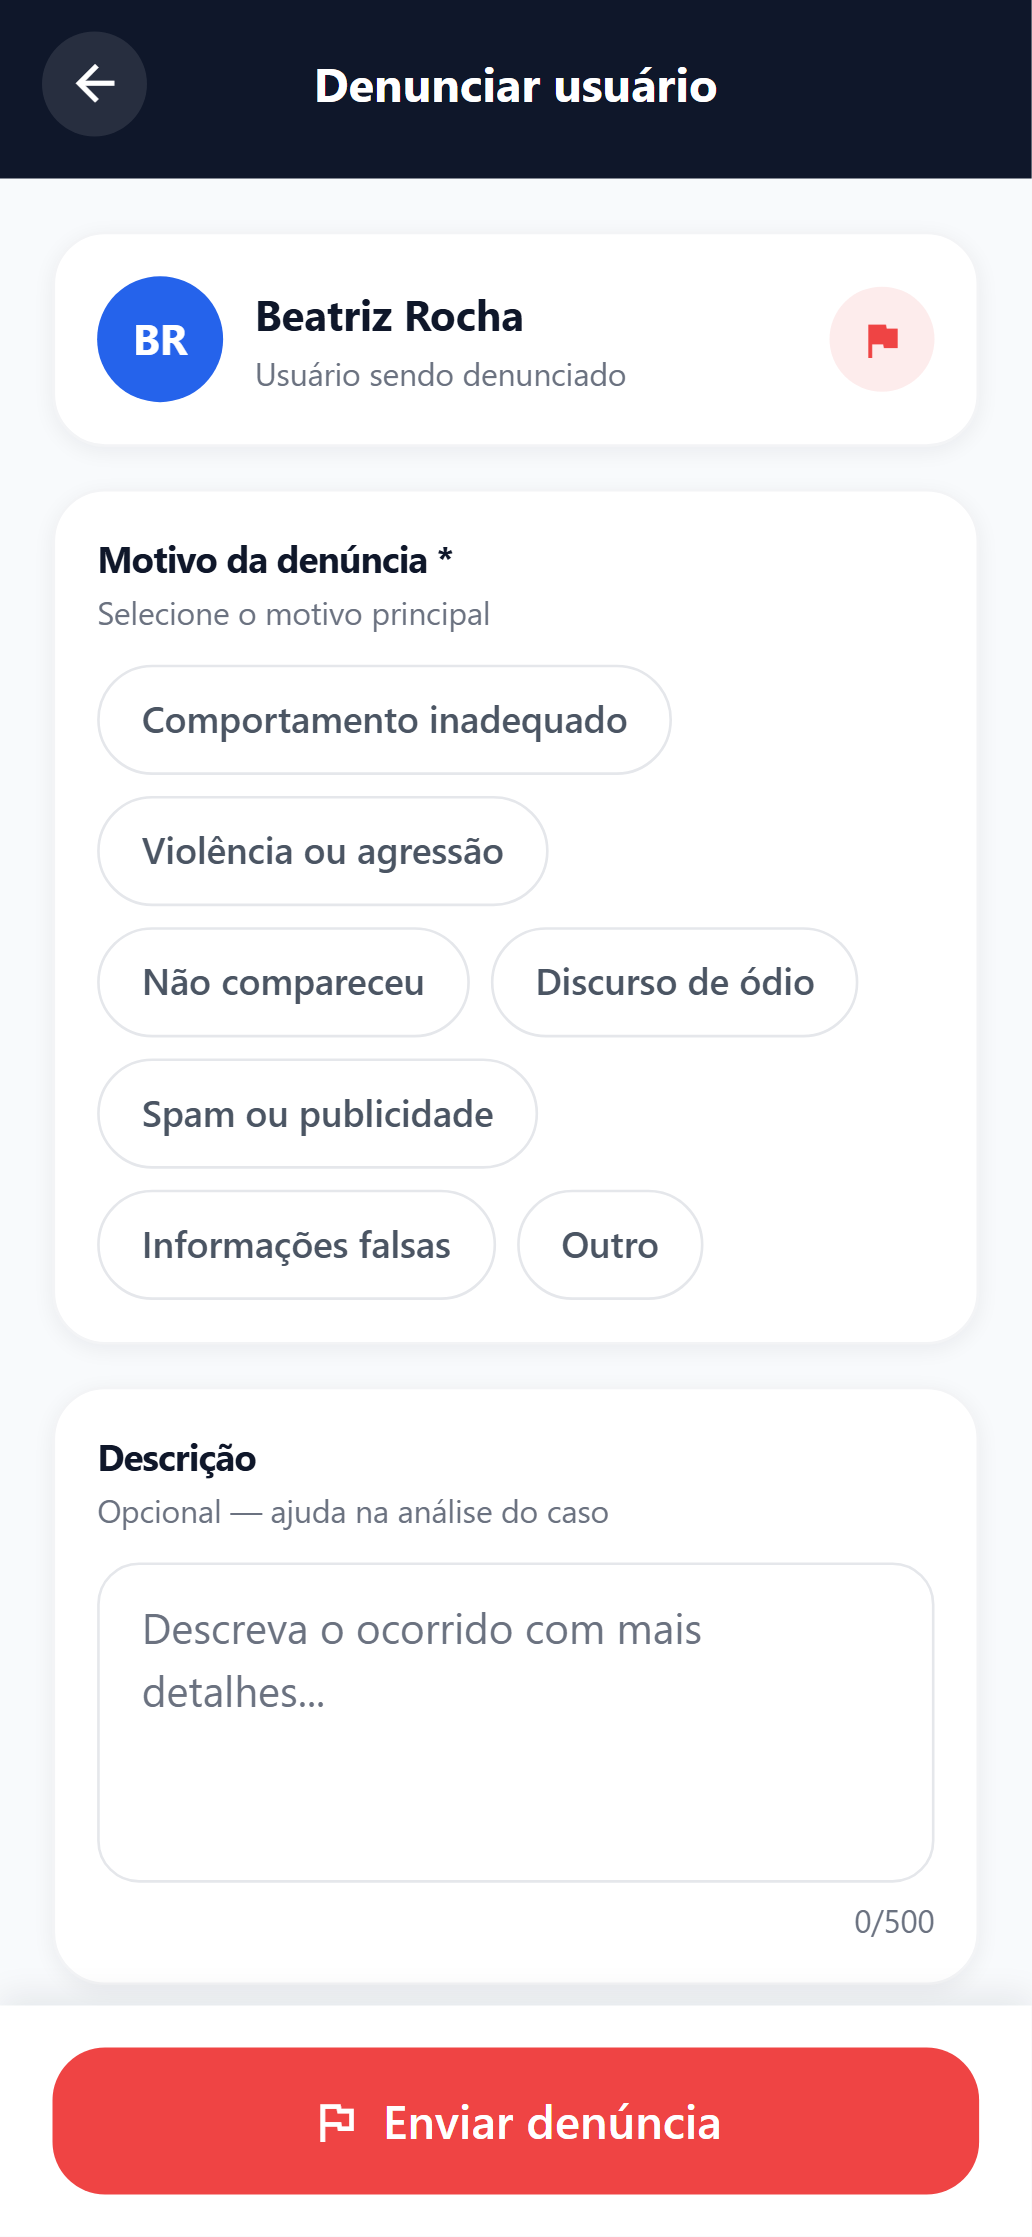
\includegraphics[width=0.32\textwidth]{assets/app/denunciar.png}
    }
    \caption{Tela de denúncia de usuário no SquadUp}
    \label{fig:app_denunciar_usuario}
\end{figure}

\subsubsection{Moderar denúncias}

Este caso de uso permite que um administrador analise as denúncias registradas pelos usuários e execute ações de moderação sobre a conta denunciada.

\textbf{Ator primário:} Administrador.

\textbf{Pré-condições:} o usuário autenticado deve possuir permissão de administrador, e deve existir ao menos uma denúncia pendente de análise.

\textbf{Pós-condições:} a denúncia passa a ter um status de resolução, e a ação de moderação correspondente é registrada.

\textbf{Fluxo principal:}

\begin{enumerate}
    \item O administrador acessa o painel administrativo;
    \item O sistema exibe a lista de denúncias pendentes de análise;
    \item O administrador seleciona uma denúncia para consultar seus detalhes, como motivo, descrição e usuário denunciado;
    \item O administrador escolhe uma ação de moderação: arquivar, advertir ou banir o usuário denunciado;
    \item O sistema registra a ação escolhida e atualiza o status da denúncia.
\end{enumerate}

\textbf{Fluxos alternativos:}

\begin{itemize}
    \item Caso o usuário autenticado não possua permissão de administrador, o sistema não disponibiliza o acesso ao painel administrativo;
    \item Caso a denúncia já tenha sido previamente resolvida, o sistema não permite uma nova ação de moderação sobre ela.
\end{itemize}

% Quando o screenshot da tela do painel administrativo estiver disponível, descomente e ajuste o caminho abaixo.
% \begin{figure}[H]
%     \centering
%     \fcolorbox{gray}{white}{
%         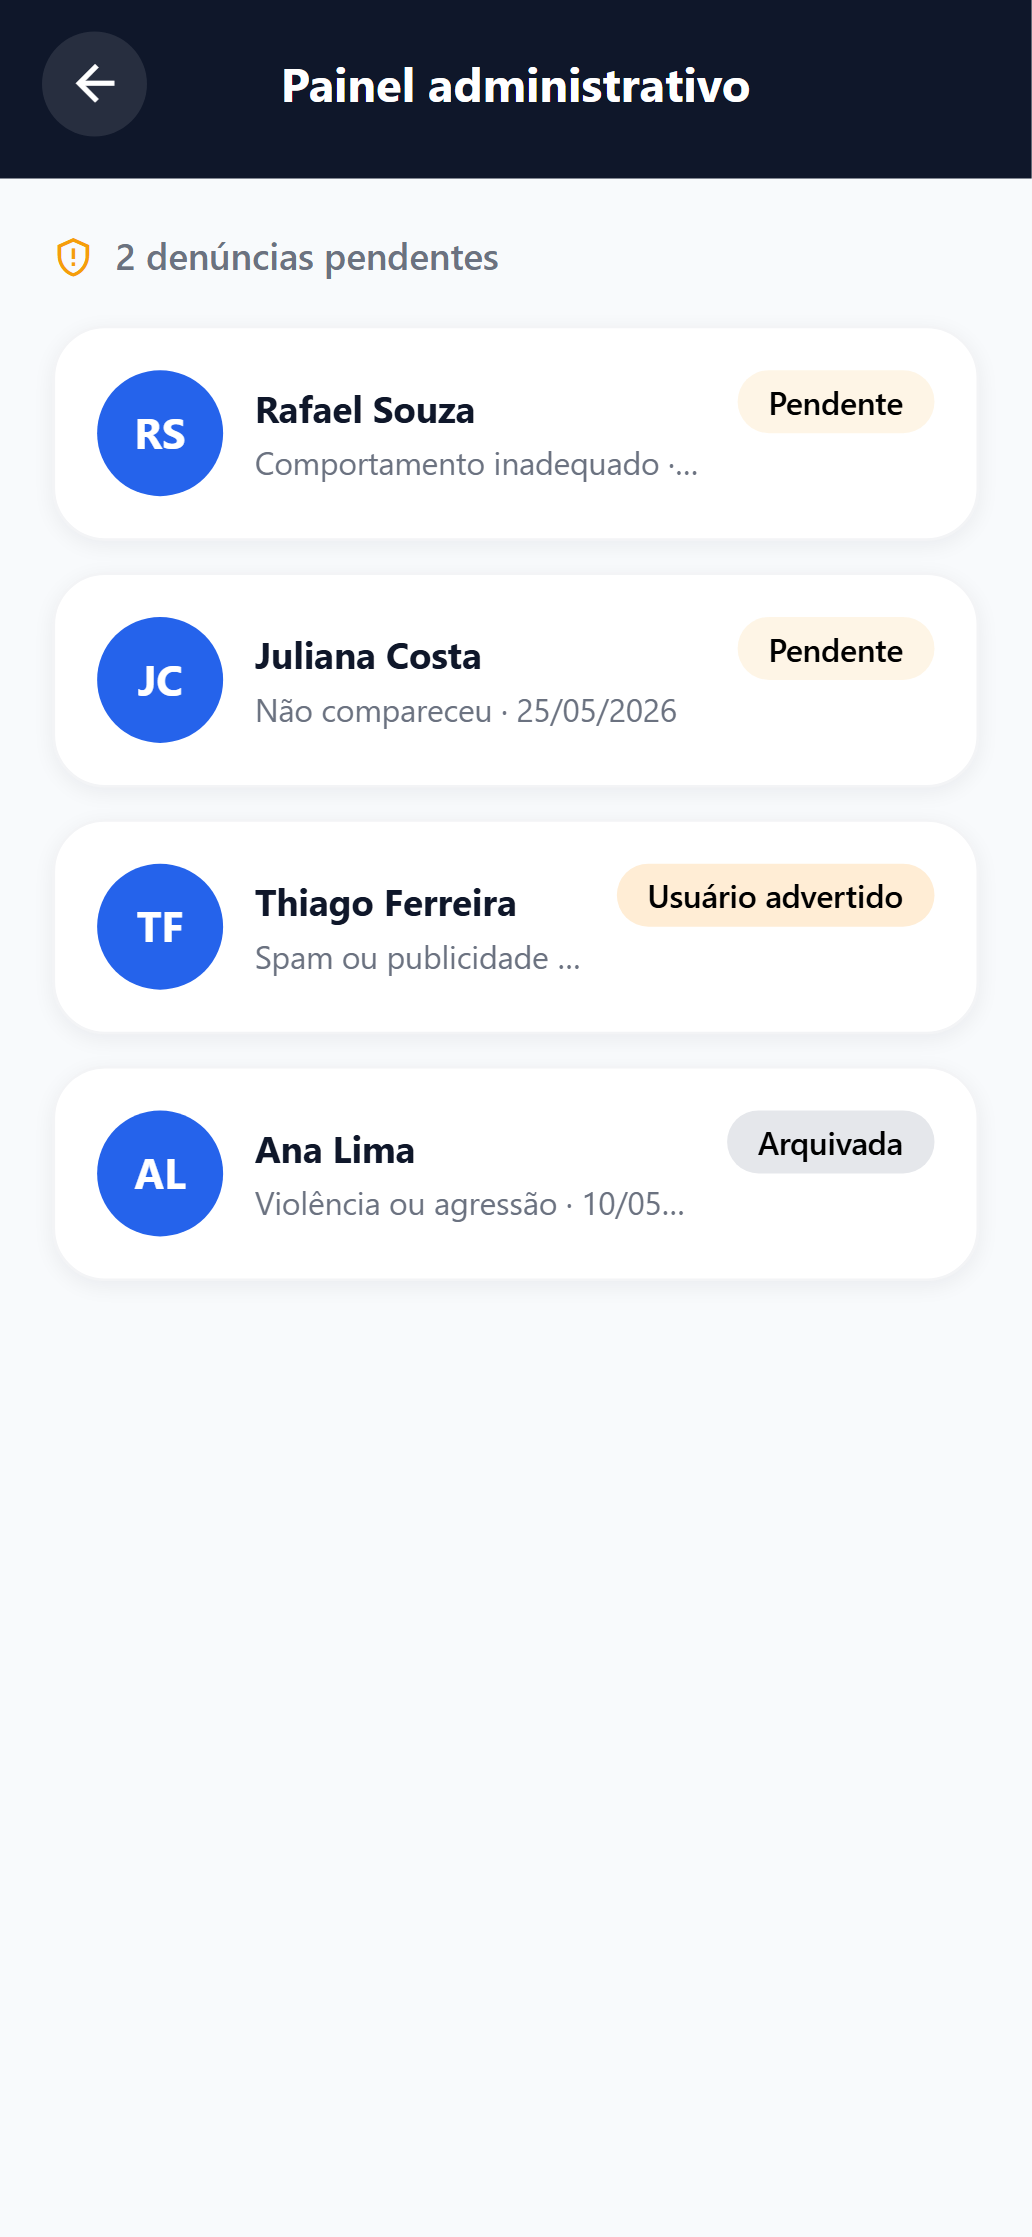
\includegraphics[width=0.32\textwidth]{assets/app/moderacao.png}
%     }
%     \caption{Painel administrativo de moderação de denúncias no SquadUp}
%     \label{fig:app_moderacao}
% \end{figure}

\subsection{Telas e fluxos da aplicação}

As telas apresentadas nesta seção foram definidas a partir dos casos de uso priorizados e representam os principais pontos de interação do usuário com o SquadUp. O fluxo geral da aplicação permite que o usuário se autentique, encontre uma partida na tela inicial, consulte seus detalhes, confirme participação, converse com os demais participantes, visualize informações de outros participantes, avalie-os após a partida, crie novas partidas e utilize mecanismos de denúncia quando necessário.

A tela de login concentra o acesso à aplicação, seja por um usuário já cadastrado, seja por um usuário recém-criado a partir do fluxo de cadastro. A tela inicial concentra a descoberta de partidas disponíveis. A tela de criação permite que usuários organizem novas atividades esportivas. As telas de detalhes apresentam as informações necessárias para a decisão de participação, incluindo, para o organizador, as ações de aprovação de participantes e encerramento da partida. A tela de chat fortalece a comunicação entre participantes confirmados antes do encontro presencial. A tela de perfil fortalece o pilar social da aplicação ao permitir que usuários conheçam melhor outros participantes, enquanto a avaliação pós-partida consolida a reputação construída a partir de partidas concluídas. Por fim, as telas de denúncia e o painel administrativo de moderação representam os mecanismos de segurança da aplicação, contribuindo para a manutenção da comunidade.

\begin{figure}[H]
    \centering

    \begin{minipage}{0.28\textwidth}
        \centering
        \fcolorbox{gray}{white}{
            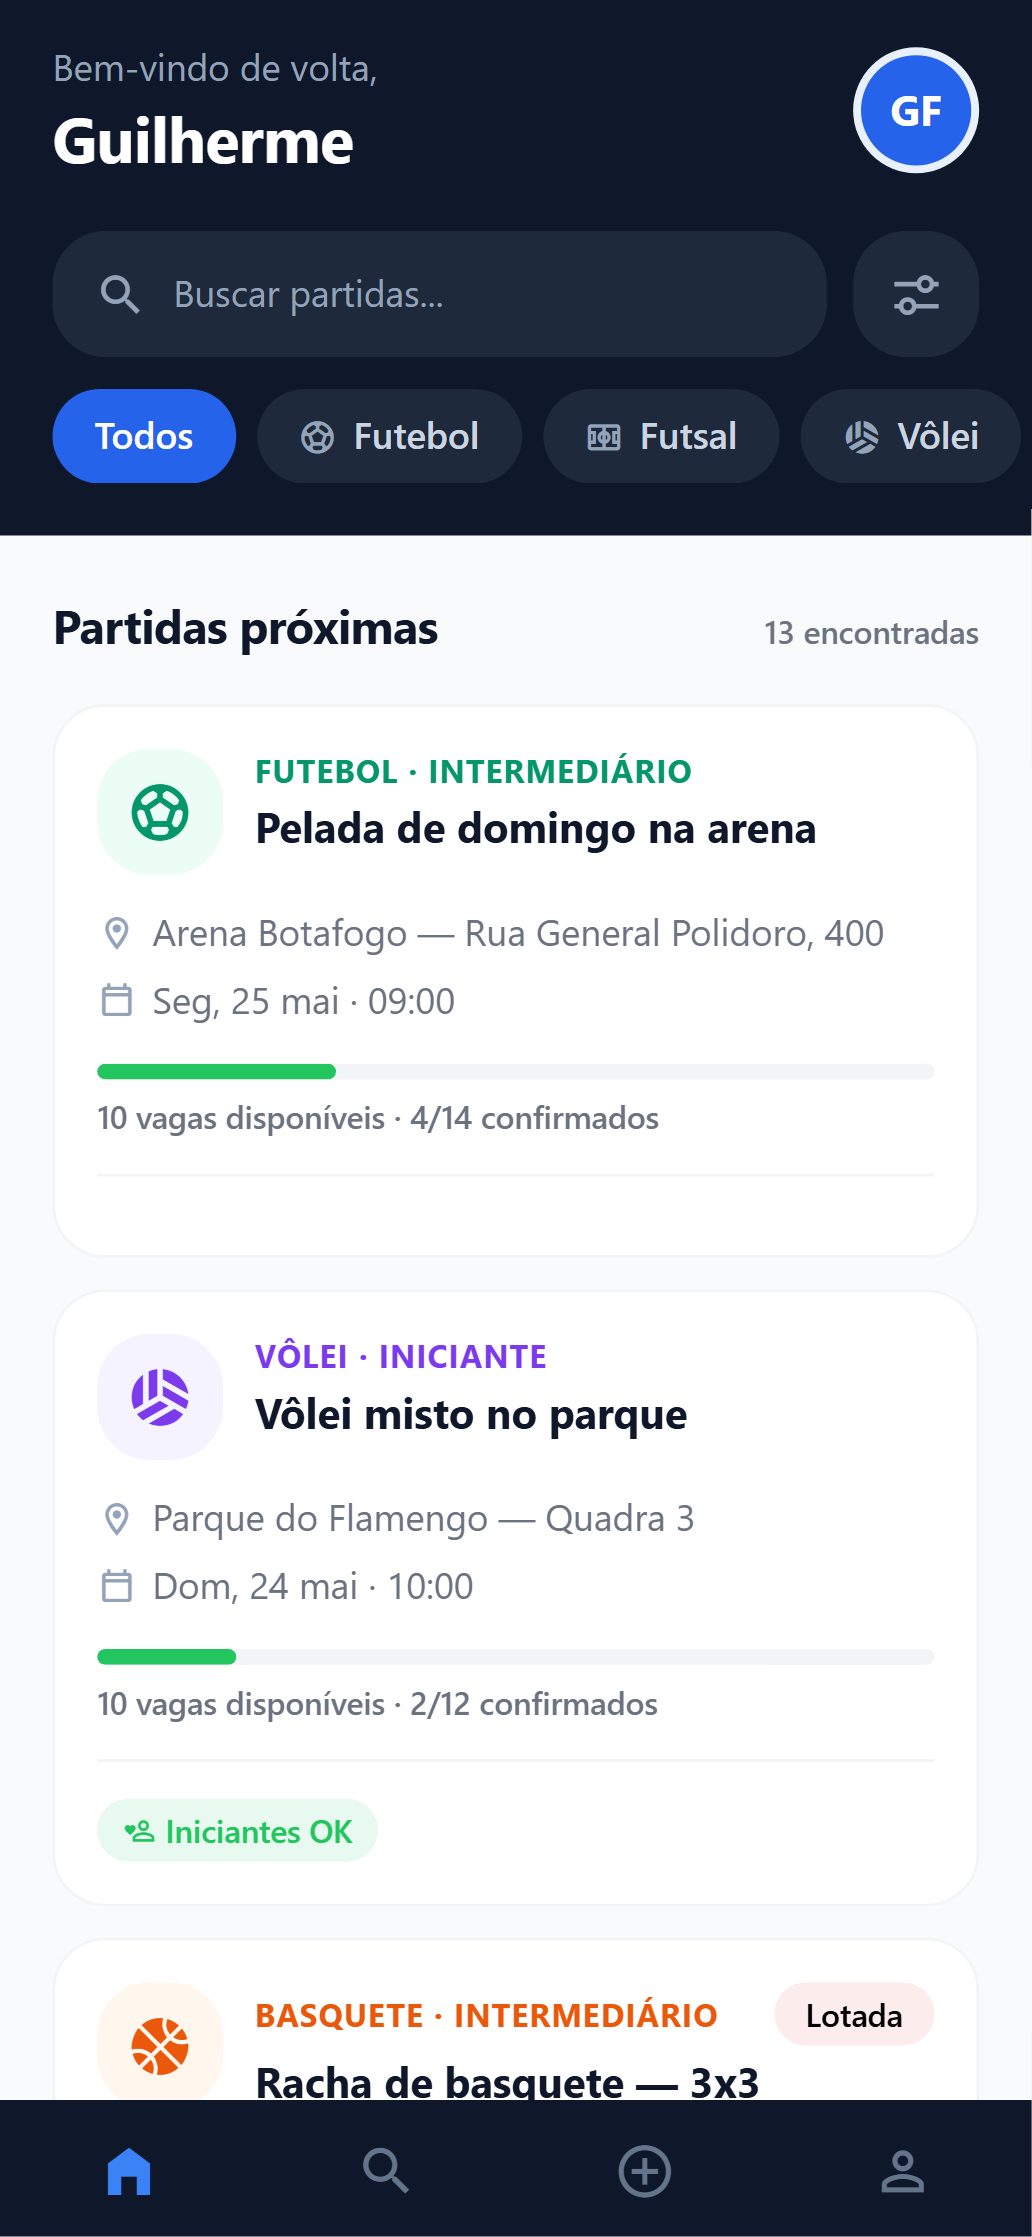
\includegraphics[width=0.95\textwidth]{assets/app/feed-principal.png}
        }
        \caption*{Feed principal}
    \end{minipage}
    \hspace{0.025\textwidth}
    \begin{minipage}{0.28\textwidth}
        \centering
        \fcolorbox{gray}{white}{
            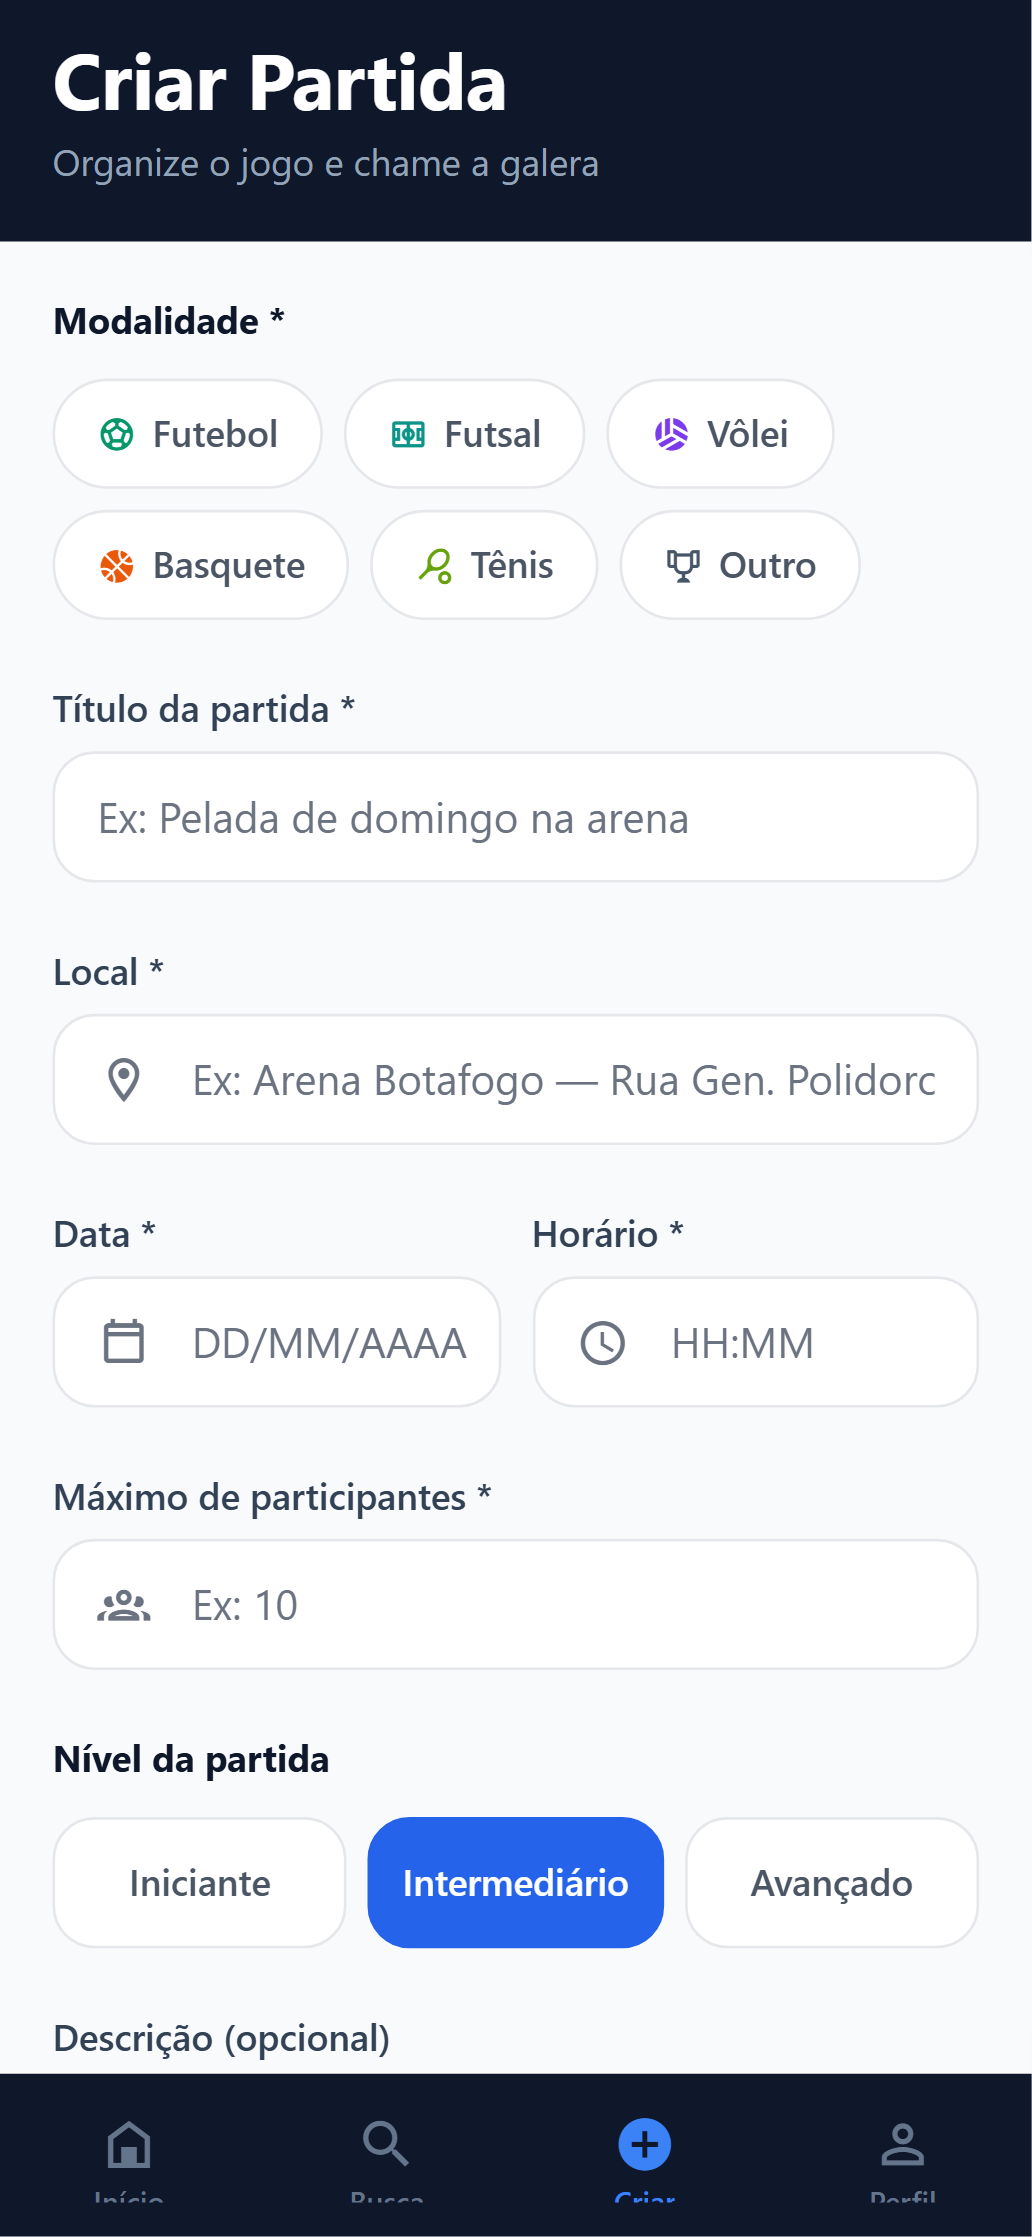
\includegraphics[width=0.95\textwidth]{assets/app/criar-partida.png}
        }
        \caption*{Criar partida}
    \end{minipage}
    \hspace{0.025\textwidth}
    \begin{minipage}{0.28\textwidth}
        \centering
        \fcolorbox{gray}{white}{
            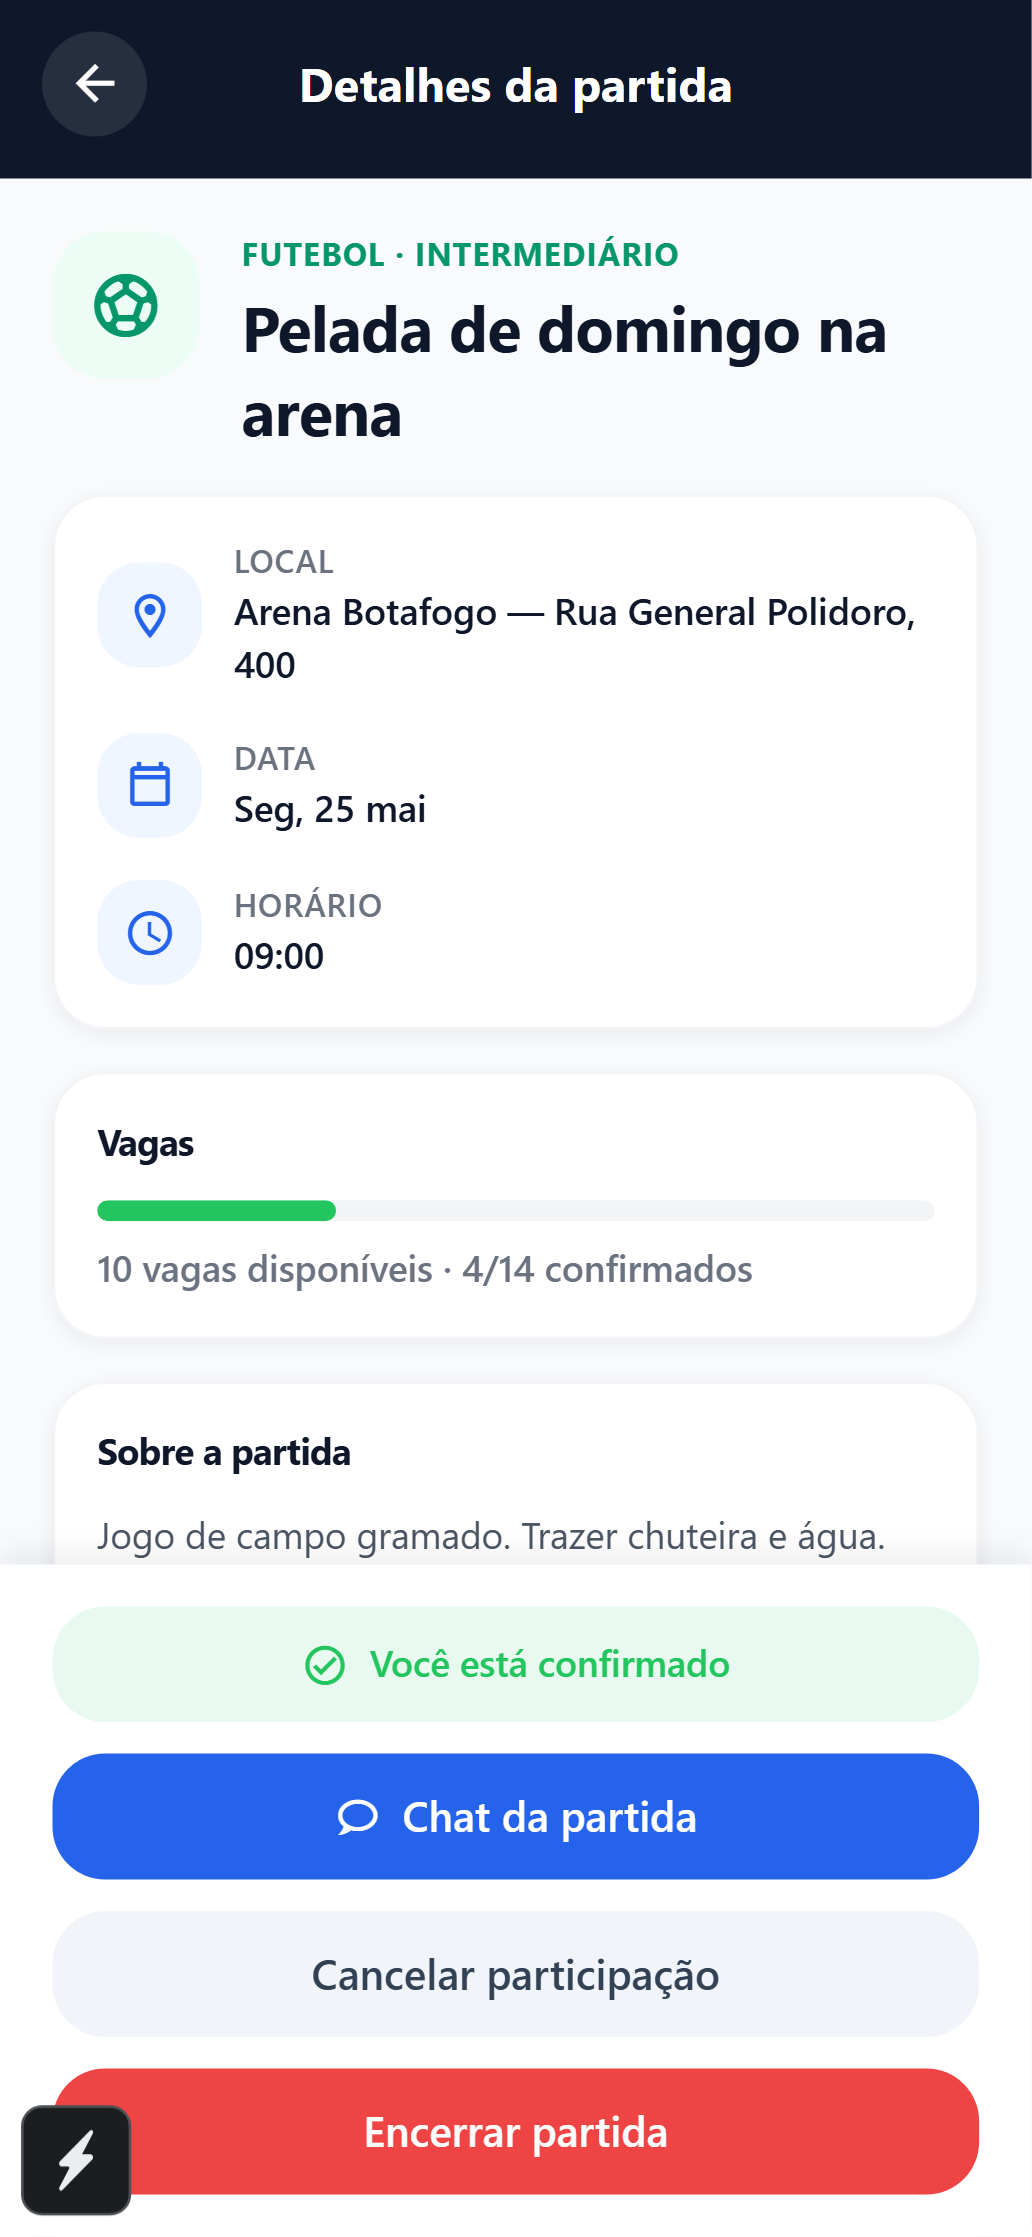
\includegraphics[width=0.95\textwidth]{assets/app/detalhes-partida.png}
        }
        \caption*{Detalhes}
    \end{minipage}

    \caption{Principais telas de descoberta, criação e visualização de partidas}
    \label{fig:app_fluxo_partidas}
\end{figure}

\begin{figure}[H]
    \centering

    \begin{minipage}{0.28\textwidth}
        \centering
        \fcolorbox{gray}{white}{
            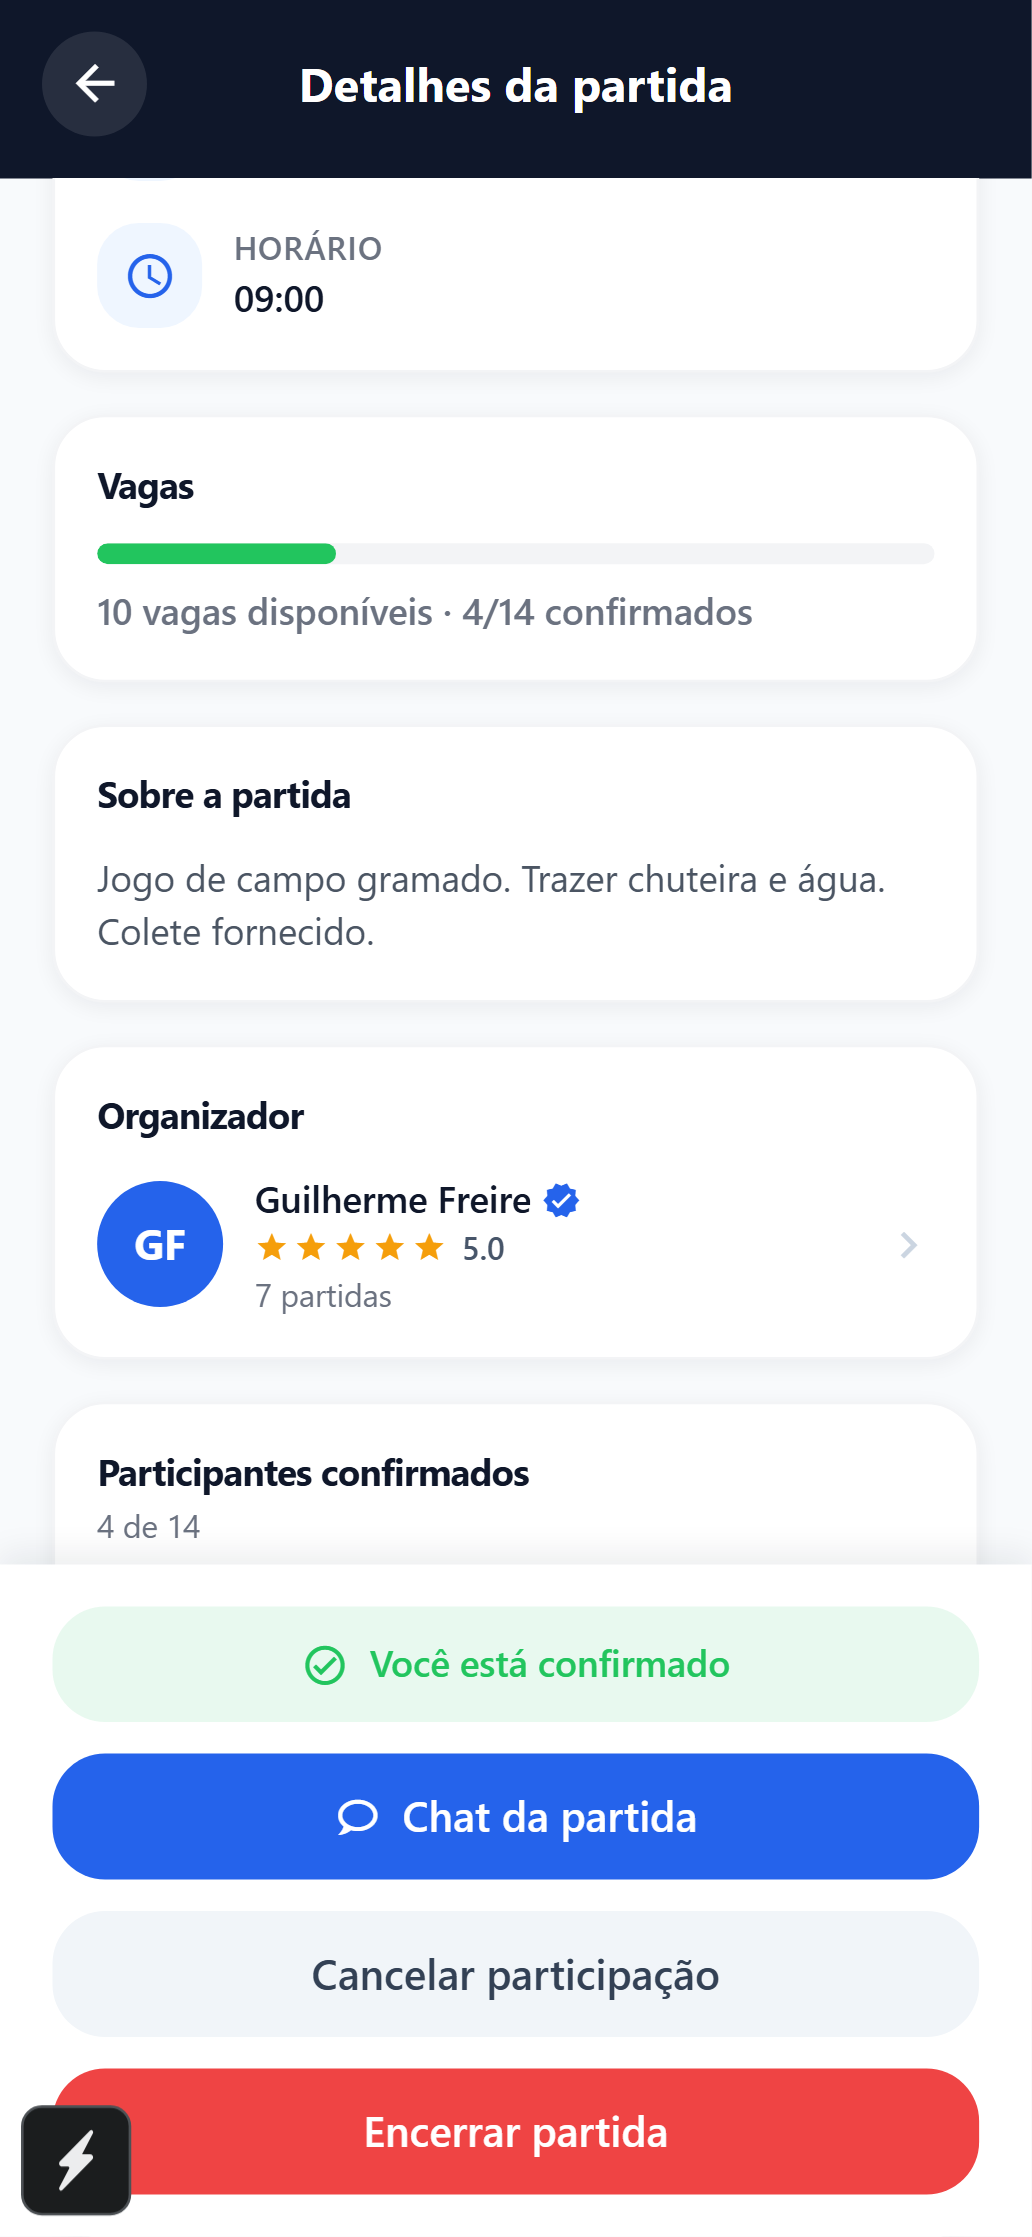
\includegraphics[width=0.95\textwidth]{assets/app/detalhes-partida-2.png}
        }
        \caption*{Detalhes complementares}
    \end{minipage}
    \hspace{0.025\textwidth}
    \begin{minipage}{0.28\textwidth}
        \centering
        \fcolorbox{gray}{white}{
            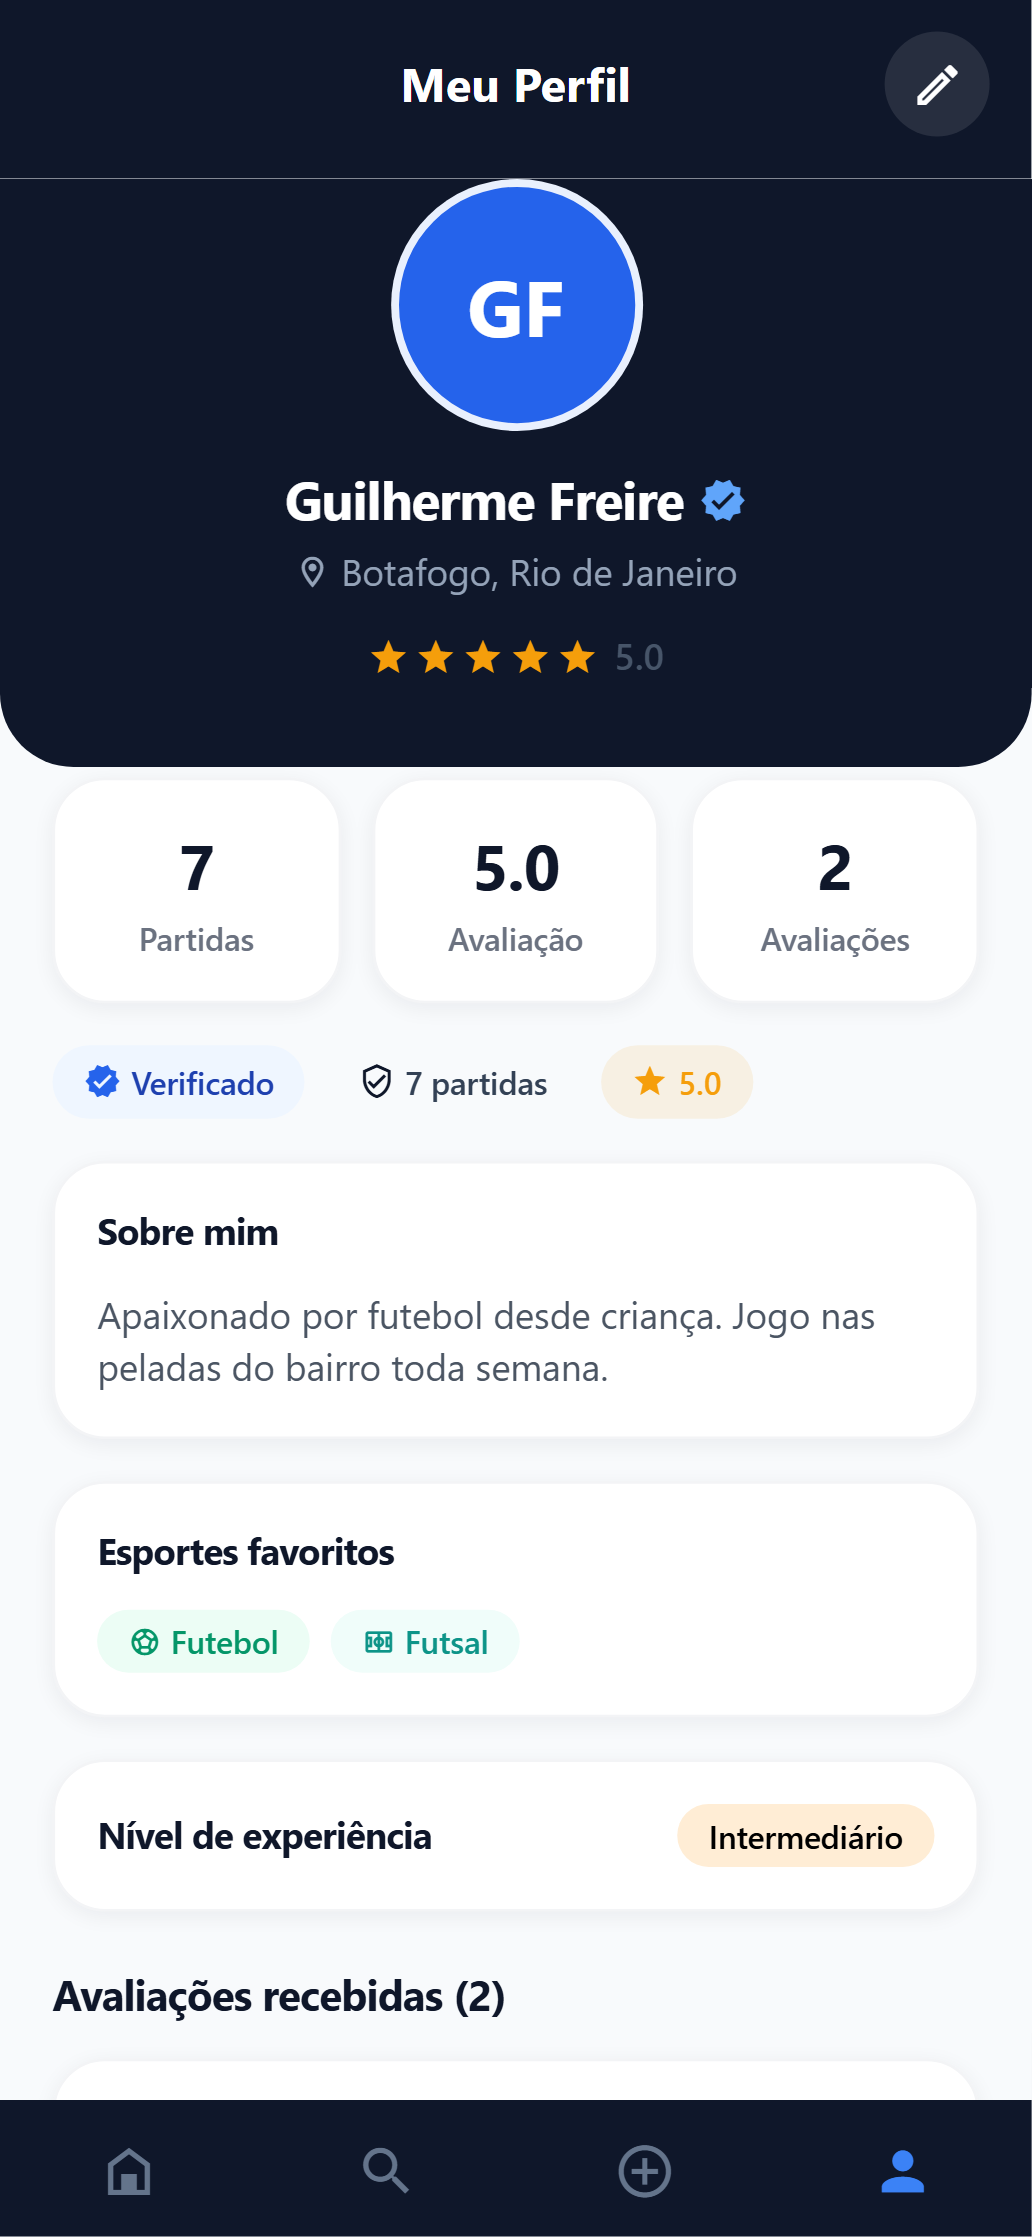
\includegraphics[width=0.95\textwidth]{assets/app/perfil.png}
        }
        \caption*{Perfil}
    \end{minipage}
    \hspace{0.025\textwidth}
    \begin{minipage}{0.28\textwidth}
        \centering
        \fcolorbox{gray}{white}{
            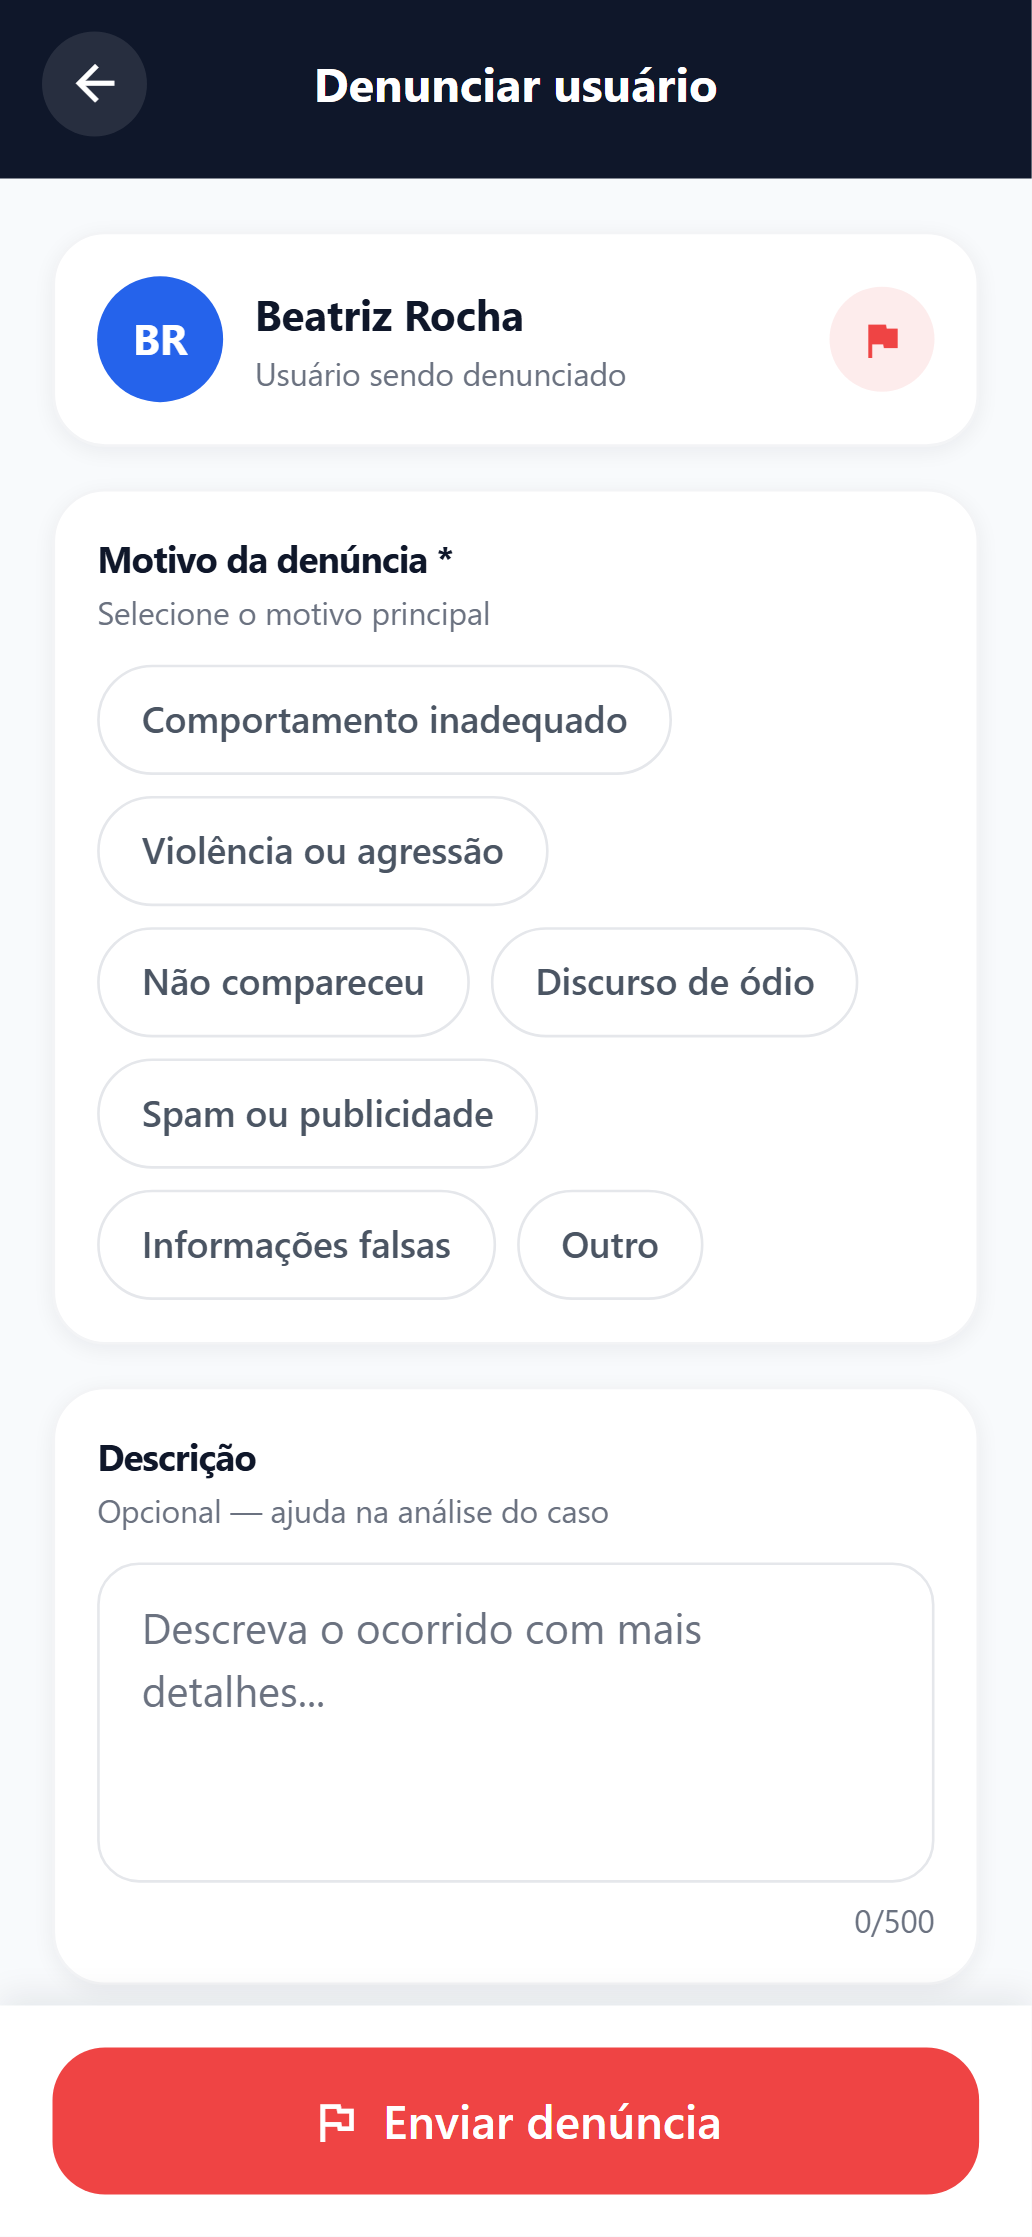
\includegraphics[width=0.95\textwidth]{assets/app/denunciar.png}
        }
        \caption*{Denúncia}
    \end{minipage}

    \caption{Telas relacionadas à participação, confiança e segurança}
    \label{fig:app_fluxo_confianca}
\end{figure}

\subsection{Considerações finais}

O desenvolvimento funcional apresentado nesta seção consolida os principais fluxos do SquadUp. A definição dos pilares do sistema, dos atores, dos casos de uso e das telas permite demonstrar como a aplicação busca reduzir barreiras sociais e logísticas para a prática de esportes coletivos. Os casos de uso descritos cobrem o ciclo completo de uso da aplicação: autenticação, descoberta e criação de partidas, participação (incluindo seu cancelamento e a aprovação de solicitações pelo organizador), comunicação entre participantes, construção de reputação por meio de avaliações e os mecanismos de segurança da comunidade, materializados na denúncia de usuários e na moderação administrativa. As telas apresentadas evidenciam o fluxo central do sistema, desde a descoberta de partidas até os mecanismos de confiança e segurança entre usuários.

\clearpage

\section{Arquitetura Tecnológica}

Esta seção apresenta a arquitetura tecnológica do SquadUp, reunindo os conceitos técnicos necessários para a compreensão da solução, as tecnologias adotadas, a organização cliente-servidor, as camadas do sistema e as principais entidades previstas.

\subsection{Conceitos fundamentais}

Esta subseção apresenta os principais conceitos técnicos utilizados ao longo deste trabalho. O objetivo é fornecer uma base de entendimento para leitores que não possuem familiaridade com desenvolvimento de software, aplicações móveis ou arquitetura de sistemas.

\subsubsection{Aplicativos móveis}

Aplicativos móveis são programas desenvolvidos para dispositivos móveis, como smartphones e tablets. Diferentemente de aplicações executadas em navegadores web, aplicativos móveis podem utilizar recursos específicos do dispositivo, como câmera, GPS, notificações e armazenamento local.

No contexto deste trabalho, o SquadUp foi concebido como um aplicativo móvel, permitindo que os usuários encontrem e organizem partidas esportivas diretamente por meio de seus dispositivos.

\subsubsection{Frontend}

Frontend corresponde à camada visual de uma aplicação. É a parte do sistema com a qual os usuários interagem diretamente por meio de telas, botões, formulários e demais elementos gráficos.

No SquadUp, o frontend é responsável por apresentar informações sobre partidas, usuários, avaliações e demais funcionalidades disponíveis.

\subsubsection{Backend}

Backend corresponde à camada responsável pelo processamento das regras de negócio da aplicação. Essa camada recebe solicitações dos usuários, executa validações, processa informações e interage com o banco de dados.

No SquadUp, o backend é responsável por funcionalidades como cadastro de usuários, gerenciamento de partidas, controle de participações, avaliações e denúncias.

\subsubsection{API REST}

Uma API (\textit{Application Programming Interface}) consiste em um conjunto de mecanismos que permite a comunicação entre diferentes sistemas.

No modelo REST (\textit{Representational State Transfer}), essa comunicação ocorre por meio de requisições realizadas pela internet. Dessa forma, o aplicativo móvel envia solicitações à API e recebe informações processadas pelo servidor.

No SquadUp, a API atua como intermediária entre o aplicativo móvel e o banco de dados.

\subsubsection{React Native}

React Native é um framework utilizado para desenvolvimento de aplicações móveis multiplataforma. Sua principal característica é permitir que um único código-fonte seja utilizado para gerar aplicações compatíveis com Android e iOS.

A escolha do React Native para este projeto foi motivada pela ampla adoção da tecnologia e pela possibilidade de desenvolvimento multiplataforma.

\subsubsection{FastAPI}

FastAPI é um framework para desenvolvimento de APIs utilizando a linguagem Python. A ferramenta oferece recursos para definição de rotas, validação de dados, autenticação e documentação automática de serviços.

Neste trabalho, o FastAPI foi utilizado para implementação da camada de backend do sistema.

\subsubsection{PostgreSQL}

PostgreSQL é um sistema gerenciador de banco de dados relacional amplamente utilizado em aplicações corporativas e acadêmicas.

Sua função consiste em armazenar e organizar informações de forma persistente, permitindo consultas, atualizações e manutenção da integridade dos dados.

No SquadUp, o PostgreSQL foi utilizado para armazenar usuários, partidas, participações, avaliações e denúncias.

\subsubsection{Geolocalização}

Geolocalização é o processo de identificação da posição geográfica de um dispositivo por meio de coordenadas de latitude e longitude.

Essa tecnologia permite que aplicações identifiquem locais próximos ao usuário e ofereçam funcionalidades baseadas em proximidade geográfica.

No SquadUp, a geolocalização foi utilizada para facilitar a descoberta de partidas esportivas próximas ao usuário. As coordenadas são obtidas a partir do GPS do próprio dispositivo, tanto no momento da criação de uma partida quanto no momento da busca, quando o usuário opta por filtrar partidas por proximidade e define um raio de busca. A distância entre o usuário e cada partida é calculada no servidor e exibida diretamente na listagem. A funcionalidade é aditiva: o campo textual de local permanece sempre obrigatório, e a recusa da permissão de localização pelo usuário não impede a criação de partidas nem a realização de buscas, apenas remove o filtro por proximidade.

\subsubsection{Notificações push}

Notificações \textit{push} são mensagens enviadas por um servidor e exibidas diretamente pelo sistema operacional do dispositivo, mesmo quando o aplicativo não está em primeiro plano. Esse recurso permite que o usuário seja avisado de eventos relevantes sem a necessidade de manter a aplicação aberta.

No SquadUp, notificações \textit{push} são utilizadas para avisar o usuário sobre três eventos considerados essenciais para os pilares social e logístico do sistema: o recebimento de uma nova mensagem em uma partida da qual participa, a aprovação de uma solicitação de participação pendente e o encerramento de uma partida pelo organizador. Ao tocar em uma notificação, o usuário é encaminhado diretamente para a tela correspondente ao evento. Assim como a geolocalização, o recurso é aditivo: a recusa da permissão de notificações pelo usuário não compromete nenhum fluxo funcional da aplicação, apenas deixa de emitir o aviso do sistema operacional.

\subsubsection{Arquitetura cliente-servidor}

A arquitetura cliente-servidor é um modelo amplamente utilizado em sistemas distribuídos.

Nesse modelo, o cliente representa a aplicação utilizada pelo usuário, enquanto o servidor concentra o processamento das regras de negócio e o acesso aos dados.

No SquadUp, o aplicativo móvel atua como cliente, enquanto a API desenvolvida em FastAPI atua como servidor responsável pela comunicação com o banco de dados.

\begin{figure}[H]
    \centering
    \fbox{
        \begin{minipage}{0.6\textwidth}
            \centering
            Aplicativo Mobile\\
            $\downarrow$\\
            API REST\\
            $\downarrow$\\
            Banco de Dados
        \end{minipage}
    }
    \caption{Representação simplificada da arquitetura cliente-servidor}
    \label{fig:cliente_servidor}
\end{figure}

\subsection{Arquitetura proposta}

A arquitetura proposta para o SquadUp segue o modelo cliente-servidor, organizada em três camadas principais: apresentação, aplicação e dados. Essa divisão foi escolhida por permitir separação de responsabilidades, facilitar a manutenção do sistema e permitir evolução independente entre aplicativo \textit{mobile}, API e banco de dados.

% Quando o diagrama estiver pronto, descomente e ajuste o caminho abaixo.
% \begin{figure}[H]
%     \centering
%     \includegraphics[width=0.9\textwidth]{assets/arquitetura.png}
%     \caption{Arquitetura proposta para o SquadUp}
%     \label{fig:arquitetura}
% \end{figure}

\subsubsection{Camada de apresentação}

A camada de apresentação será composta por um aplicativo \textit{mobile} desenvolvido em React Native. Essa camada será responsável pela interface com o usuário, pela navegação entre telas e pela comunicação com os serviços disponibilizados pela API. O aplicativo contempla telas como cadastro, login, perfil, listagem de partidas, detalhes da partida, criação de partida, conversa da partida, avaliação de usuários e denúncia.

\subsubsection{Camada de aplicação}

A camada de aplicação será implementada utilizando FastAPI. Essa camada será responsável por expor uma API REST para comunicação com o aplicativo \textit{mobile}, além de centralizar as regras de negócio do sistema. Entre suas responsabilidades estão o gerenciamento de usuários, criação e busca de partidas, registro de participação, avaliações, denúncias e controle de permissões.

\subsubsection{Camada de dados}

A camada de dados será composta por um banco de dados relacional PostgreSQL. Essa escolha se justifica pela natureza estruturada das principais informações do sistema, como usuários, partidas, participações, avaliações, denúncias e locais. O modelo relacional permite representar adequadamente os vínculos entre usuários e partidas, além de facilitar consultas envolvendo filtros, histórico e reputação.

\subsection{Principais entidades}

Com base nos casos de uso, foram identificadas as seguintes entidades principais:

\begin{itemize}
    \item \textbf{Usuário}: representa a pessoa cadastrada no sistema, incluindo dados de identificação, autenticação, informações esportivas, preferências e reputação;
    \item \textbf{Partida}: representa um evento esportivo criado por um usuário, contendo modalidade, local, data, horário, vagas e descrição;
    \item \textbf{Participação}: registra o vínculo entre usuários e partidas, incluindo status de confirmação ou solicitação pendente;
    \item \textbf{Mensagem}: registra as mensagens trocadas entre os participantes de uma partida em seu chat;
    \item \textbf{Avaliação}: registra avaliações realizadas entre participantes após uma partida;
    \item \textbf{Denúncia}: registra relatos de comportamento inadequado para análise administrativa;
    \item \textbf{Local}: representa informações sobre o espaço onde a partida será realizada.
\end{itemize}

\subsection{Separação de responsabilidades}

A separação de responsabilidades entre as camadas busca reduzir acoplamento e facilitar a evolução do sistema. O aplicativo \textit{mobile} é responsável pela experiência do usuário e pela apresentação dos dados. A API é responsável por validar regras de negócio, processar requisições e garantir consistência das operações. O banco de dados é responsável pela persistência e integridade das informações.

\subsection{Segurança e privacidade}

A segurança da informação é um requisito relevante para o SquadUp, uma vez que o sistema lida com dados pessoais e viabiliza a interação entre usuários que, muitas vezes, não se conhecem previamente. Assim, a arquitetura do sistema incorpora um conjunto de práticas voltadas à proteção dos dados e ao controle de acesso.

A autenticação do usuário é realizada por meio de tokens \textit{JWT} (\textit{JSON Web Token}), com um mecanismo de renovação (\textit{refresh token}) que permite manter a sessão do usuário ativa sem exigir um novo login a cada acesso, ao mesmo tempo em que limita o tempo de validade de cada token individual. As senhas dos usuários nunca são armazenadas em texto plano: são processadas por meio de uma função de \textit{hash} unidirecional antes de serem persistidas no banco de dados, de modo que, mesmo em caso de acesso indevido à base de dados, as senhas originais não fiquem expostas.

O sistema também implementa controle de acesso baseado em papéis (\textit{RBAC}, \textit{Role-Based Access Control}), distinguindo usuários comuns de administradores. Ações sensíveis, como a moderação de denúncias, ficam restritas ao papel de administrador. Por fim, sessões e tokens de acesso expirados ou revogados são removidos periodicamente pelo sistema, reduzindo a superfície de dados sensíveis mantida em memória e em banco ao longo do tempo.

\subsection{Considerações finais}

A arquitetura tecnológica proposta organiza o SquadUp em camadas bem definidas, separando interface, regras de negócio e persistência de dados. Essa estrutura favorece a manutenção do sistema, facilita a evolução independente entre frontend e backend e permite representar de forma adequada as entidades centrais da aplicação. As práticas de segurança adotadas, combinadas com os mecanismos de confiança apresentados no Capítulo 3, reforçam o compromisso do SquadUp com uma experiência de conexão entre usuários desconhecidos que seja, ao mesmo tempo, simples e segura.

\clearpage

\section{Cronograma}

O desenvolvimento do projeto seguirá o cronograma apresentado na Tabela \ref{tab:cronograma}. O cronograma foi dividido em períodos quinzenais, contemplando atividades de modelagem, implementação, integração, testes, ajustes finais, revisão da monografia e preparação para a defesa.

\begin{table}[H]
\centering
\caption{Cronograma de Desenvolvimento do Projeto}
\label{tab:cronograma}
\scriptsize
\resizebox{\textwidth}{!}{
\begin{tabular}{|l|c|c|c|c|c|c|c|c|c|c|c|c|c|c|c|}
\hline
\textbf{Etapa} 
& \textbf{Mai 1} 
& \textbf{Mai 2} 
& \textbf{Jun 1} 
& \textbf{Jun 2} 
& \textbf{Jul 1} 
& \textbf{Jul 2} 
& \textbf{Ago 1} 
& \textbf{Ago 2} 
& \textbf{Set 1} 
& \textbf{Set 2} 
& \textbf{Out 1} 
& \textbf{Out 2} 
& \textbf{Nov 1} 
& \textbf{Nov 2} 
& \textbf{Dez 1} \\
\hline

Definição do tema e escopo 
& X & X &  &  &  &  &  &  &  &  &  &  &  &  &  \\
\hline

Revisão bibliográfica 
& X & X & X & X &  &  &  &  &  &  &  &  &  &  &  \\
\hline

Análise de trabalhos relacionados e concorrentes 
& X & X & X & X &  &  &  &  &  &  &  &  &  &  &  \\
\hline

Levantamento de requisitos 
&  & X & X & X &  &  &  &  &  &  &  &  &  &  &  \\
\hline

Modelagem dos casos de uso 
&  & X & X & X & X &  &  &  &  &  &  &  &  &  &  \\
\hline

Arquitetura e modelagem técnica 
&  & X & X & X & X & X &  &  &  &  &  &  &  &  &  \\
\hline

Prototipação das telas e fluxos 
&  & X & X & X & X & X &  &  &  &  &  &  &  &  &  \\
\hline

Implementação do frontend 
&  & X & X & X & X & X &  &  &  &  &  &  &  &  &  \\
\hline

Implementação do backend 
&  &  &  &  &  & X & X & X & X &  &  &  &  &  &  \\
\hline

Integração entre frontend e backend 
&  &  &  &  &  &  &  & X & X & X &  &  &  &  &  \\
\hline

Testes e validação dos fluxos 
&  &  &  &  &  &  &  &  & X & X & X &  &  &  &  \\
\hline

Validação com orientador e ajustes funcionais 
&  &  &  &  &  &  &  &  &  & X & X & X &  &  &  \\
\hline

Escrita da monografia 
&  & X & X & X & X & X & X & X & X & X & X &  &  &  &  \\
\hline

Revisão final da monografia 
&  &  &  &  &  &  &  &  &  &  & X & X & X &  &  \\
\hline

Correções finais 
&  &  &  &  &  &  &  &  &  &  &  & X & X & X &  \\
\hline

Preparação da defesa 
&  &  &  &  &  &  &  &  &  &  &  &  & X & X & X \\
\hline

Defesa do TCC 
&  &  &  &  &  &  &  &  &  &  &  &  &  &  & X \\
\hline

\end{tabular}
}
\end{table}

\clearpage

\section{Considerações Finais}

Este trabalho apresentou o SquadUp, um aplicativo \textit{mobile} voltado à conexão de usuários interessados na prática de esportes coletivos. A solução foi estruturada a partir da identificação de dificuldades relacionadas à formação de grupos, organização de partidas, confiança entre participantes e continuidade da prática esportiva.

A revisão da literatura e a análise de aplicativos similares indicaram que existem soluções voltadas a aspectos específicos do problema, como registro de atividades, organização de eventos, reserva de espaços ou comunicação em grupos. Entretanto, foi identificada uma lacuna relacionada à integração entre conexão social, organização logística e mecanismos de confiança para usuários que desejam praticar esportes coletivos com pessoas desconhecidas.

Como resultado, foram definidos os objetivos do sistema, seus pilares principais, casos de uso, arquitetura proposta, telas principais e cronograma de desenvolvimento. A proposta apresentada demonstra como o SquadUp busca integrar conexão social, organização logística e mecanismos de confiança em uma solução voltada à prática de esportes coletivos.

\end{justify}

\clearpage
\bibliographystyle{plain}
\bibliography{references}

\end{document}